% !TEX TS-program = XeLaTeX
% !TeX program = xelatex
% Command for running this example (needs latexmkrc file):
%    latexmk -bibtex -pdf main.tex

%	نمونه پایان‌نامه آماده شده با استفاده از کلاس tehran-thesis، نگارش 1
%	سینا ممکن، دانشگاه تهران 
%	https://github.com/sinamomken/tehran-thesis
%	گروه پارسی‌لاتک
%	http://www.parsilatex.com
%	این نسخه، بر اساس نسخه‌ 0.1 از کلاس IUST-Thesis آقای محمود امین‌طوسی آماده شده است.
%        http://profsite.sttu.ac.ir/mamintoosi

%----------------------------------------------------------------------------------------------
% اگر قصد نوشتن پروژه کارشناسی را دارید، در خط زیر به جای msc، کلمه bsc و اگر قصد نوشتن رساله دکترا را دارید، کلمه phd را قرار دهید. کلیه تنظیمات لازم، به طور خودکار، اعمال می‌شود.

% اگر مایلید پایان‌نامه شما دورو باشد به جای oneside در خط زیر از twoside استفاده کنید.

% برای حاشیه‌نویسی و کم کردن صفحات ابتدایی، گزینه draft را وارد و برای نسخه نهایی آن را حذف کنید.

% برای استفاده از قلم‌های سری IR Series گزینه irfonts را وارد و برای استفاده از قلم‌های X Series 2 آن را حذف کنید.

\documentclass[
twoside
% ,openany
,msc
,irfonts
% ,draft
]{./tex/tehran-thesis}

% فایل commands.tex را مطالعه کنید؛ چون دستورات مربوط به فراخوانی بسته‌ها، فونت و دستورات خاص در این فایل قرار دارد.
% در این فایل، دستورها و تنظیمات مورد نیاز، آورده شده است.
%-------------------------------------------------------------------------------------------------------------------
% دستوراتی که پوشه پیش‌فرض زیرفایل‌های tex را مشخص می‌کند.
%\makeatletter
%\def\input@path{{./tex/}}
%\makeatother
% در ورژن جدید زی‌پرشین برای تایپ متن‌های ریاضی، این سه بسته، حتماً باید فراخوانی شود
\usepackage{amsthm,amssymb,amsmath}
% بسته‌ای برای تنطیم حاشیه‌های بالا، پایین، چپ و راست صفحه
\usepackage[a4paper, top=35mm, bottom=25mm, left=25mm, right=35mm]{geometry}
% بسته‌‌ای برای ظاهر شدن شکل‌ها و تعیین آدرس تصاویر
\usepackage[final]{graphicx}
\graphicspath{{./img/}}
% بسته‌های مورد نیاز برای نوشتن کدها، رنگ‌آمیزی آنها و تعیین پوشهٔ کدها
\usepackage[final]{listings}
\usepackage[usenames,dvipsnames,svgnames,table]{xcolor}
\lstset{inputpath=./code/}
% بسته‌ای برای رسم کادر
\usepackage{framed} 
% بسته‌‌ای برای چاپ شدن خودکار تعداد صفحات در صفحه «معرفی پایان‌نامه»
\usepackage{lastpage}
% بسته‌ٔ لازم برای: ۱. تغییر شماره‌گذاری صفحات پیوست. ۲. تصحیح باگ آدرس وب حاوی '%' در مراجع
\usepackage{etoolbox}

%%%%%%%%%%%%%%%%%%%%%%%%%%%%%%%%%%%%
%%% دستورات وابسته به استیل مراجع:
%% اگر از استیل‌های natbib (plainnat-fa، asa-fa، chicago-fa) استفاده می‌کنید، خط زیر را فعال و بعدی‌اش را غیرفعال کنید.
%\usepackage{natbib}
%\newcommand{\citelatin}[1]{\cite{#1}\LTRfootnote{\citeauthor*{#1}}}
%\newcommand{\citeplatin}[1]{\citep{#1}\LTRfootnote{\citeauthor*{#1}}}
%% اگر از سایر استیل‌ها استفاده می‌کنید، خط بالا را غیرفعال و خط‌های زیر را فعال کنید.
\let\citep\cite
\let\citelatin\cite
\let\citeplatin\cite
%%%%%%%%%%%%
% بررسی حالت پیش نویس
\usepackage{ifdraft}
\ifdraft
{%
	% بسته‌ٔ ایجاد لینک‌های رنگی با امکان جهش
	\usepackage[unicode=true,pagebackref=true,
colorlinks,linkcolor=blue,citecolor=blue,final]{hyperref}
	%\usepackage{todonotes}
	\usepackage[firstpage]{draftwatermark}
	\SetWatermarkText{\ \ \ پیش‌نویس}
	\SetWatermarkScale{1.2}
}
{ 
	\usepackage[pagebackref=false]{hyperref}
	%\usepackage[disable]{todonotes} % final without TODOs
}

\usepackage[obeyDraft]{todonotes}
\setlength{\marginparwidth}{2cm}

%%%%%%%%%%%%
%%% تصحیح باگ: اگر در مراجع، آدرس وب حاوی '%' بوده و pagebackref فعال باشد، دستورات زیر باید بیایند:
%% برای استیل‌های natbib مثل plainnat-fa، asa-fa، chicago-fa
\makeatletter
\let\ORIG@BR@@lbibitem\BR@@lbibitem
\apptocmd\ORIG@BR@@lbibitem{\endgroup}{}{}
\def\BR@@lbibitem{\begingroup\catcode`\%=12 \ORIG@BR@@lbibitem}
\makeatother
%% برای سایر استیل‌ها
\makeatletter
\let\ORIG@BR@@bibitem\BR@@bibitem
\apptocmd\ORIG@BR@@bibitem{\endgroup}{}{}
\def\BR@@bibitem{\begingroup\catcode`\%=12 \ORIG@BR@@bibitem}
\makeatother
%%%%%%%%%%%%%%%%%%%%%%%%%%%%%%%%%%%%

% بسته‌ لازم برای تنظیم سربرگ‌ها
\usepackage{fancyhdr}
%\usepackage{enumitem}
\usepackage{setspace}
% بسته‌های لازم برای نوشتن الگوریتم
\usepackage{algorithm}
\usepackage{algorithmic}
% بسته‌های لازم برای رسم بهتر جداول
\usepackage{tabulary}
\usepackage{tabularx}
\usepackage{rotating}
% بسته‌های لازم برای رسم تنظیم بهتر شکل‌ها و زیرشکل‌ها
\usepackage[export]{adjustbox}
\usepackage{subfig}
\usepackage[subfigure]{tocloft}
% بسته‌ای برای رسم نمودارها و نیز صفحه مالکیت اثر
\usepackage{tikz}
% بسته‌ای برای ظاهر شدن «مراجع» و «نمایه» در فهرست مطالب
\usepackage[nottoc]{tocbibind}
% دستورات مربوط به ایجاد نمایه
\usepackage{makeidx}
\makeindex
%%% بسته ایجاد واژه‌نامه با xindy
\usepackage[xindy,toc,acronym,nonumberlist=true]{glossaries}

% بسته‌ای برای افزودن تورفتگی به ابتدای اولین پاراگراف هر بخش
\usepackage{indentfirst}

% بسته زیر باگ ناشی از فراخوانی بسته‌های زیاد را برطرف می‌کند.
\usepackage{morewrites}
%%%%%%%%%%%%%%%%%%%%%%%%%%
% فراخوانی بسته زی‌پرشین (باید آخرین بسته باشد)
\usepackage[extrafootnotefeatures, localise=on, displaymathdigits=persian]{xepersian}




\makeatletter
% تعریف قلم فارسی و انگلیسی و مکان قلم‌ها
\if@irfonts
\settextfont[Path={./font/}, BoldFont={IRLotusICEE_Bold.ttf}, BoldItalicFont={IRLotusICEE_BoldIranic.ttf}, ItalicFont={IRLotusICEE_Iranic.ttf},Scale=1.2]{IRLotusICEE.ttf}
% LiberationSerif or FreeSerif as free equivalents of Times New Roman
\setlatintextfont[Path={./font/}, BoldFont={LiberationSerif-Bold.ttf}, BoldItalicFont={LiberationSerif-BoldItalic.ttf}, ItalicFont={LiberationSerif-Italic.ttf},Scale=1]{LiberationSerif-Regular.ttf}
% چنانچه می‌خواهید اعداد در فرمول‌ها، انگلیسی باشد، خط زیر را غیرفعال کنید
% و گزینهٔ displaymathdigits=persian را از خط ۱۰۹ حذف کنید.
\setdigitfont[Path={./font/}, Scale=1.2]{IRLotusICEE.ttf}
% تعریف قلم‌های فارسی و انگلیسی اضافی برای استفاده در بعضی از قسمت‌های متن
\setiranicfont[Path={./font/}, Scale=1.3]{IRLotusICEE_Iranic.ttf}				% ایرانیک، خوابیده به چپ
\setmathsfdigitfont[Path={./font/}]{IRTitr.ttf}
\defpersianfont\titlefont[Path={./font/}, Scale=1]{IRTitr.ttf}
% برای تعریف یک قلم خاص عنوان لاتین، خط بعد را فعال و ویرایش کنید و خط بعد از آن را غیرفعال کنید.
% \deflatinfont\latintitlefont[Scale=1]{LiberationSerif}
\font\latintitlefont=cmssbx10 scaled 2300 %cmssbx10 scaled 2300
\else
\settextfont{XB Niloofar}
\setlatintextfont{Junicode}
% چنانچه می‌خواهید اعداد در فرمول‌ها، انگلیسی باشد، خط زیر را غیرفعال کنید
% و گزینهٔ displaymathdigits=persian را از خط ۱۰۹ حذف کنید.
\setdigitfont{XB Niloofar}
% تعریف قلم‌های فارسی و انگلیسی اضافی برای استفاده در بعضی از قسمت‌های متن
% \setmathsfdigitfont{XB Titre}
\defpersianfont\titlefont{XB Titre}
\deflatinfont\latintitlefont[Scale=1.1]{Junicode}
\fi
\makeatother

% برای استفاده از قلم نستعلیق خط بعد را فعال کنید.
% \defpersianfont\nastaliq[Scale=1.2]{IranNastaliq}


%%%%%%%%%%%%%%%%%%%%%%%%%%
% راستچین شدن todonotes
\presetkeys{todonotes}{align=right,textdirection=righttoleft}{}
\makeatletter
\providecommand\@dotsep{5}
\def\listtodoname{فهرست کارهای باقیمانده}
\def\listoftodos{\noindent{\Large\vspace{10mm}\textbf{\listtodoname}}\@starttoc{tdo}}
\renewcommand{\@todonotes@MissingFigureText}{شکل}
\renewcommand{\@todonotes@MissingFigureUp}{شکل}
\renewcommand{\@todonotes@MissingFigureDown}{جاافتاده}
\makeatother
% دستوری برای حذف کلمه «چکیده»
\renewcommand{\abstractname}{}
% دستوری برای حذف کلمه «abstract»
%\renewcommand{\latinabstract}{}
% دستوری برای تغییر نام کلمه «اثبات» به «برهان»
\renewcommand\proofname{\textbf{برهان}}
% دستوری برای تغییر نام کلمه «کتاب‌نامه» به «مراجع»
\renewcommand{\bibname}{مراجع}
% دستوری برای تعریف واژه‌نامه انگلیسی به فارسی
\newcommand\persiangloss[2]{#1\dotfill\lr{#2}\\}
% دستوری برای تعریف واژه‌نامه فارسی به انگلیسی 
\newcommand\englishgloss[2]{#2\dotfill\lr{#1}\\}
% تعریف دستور جدید «\پ» برای خلاصه‌نویسی جهت نوشتن عبارت «پروژه/پایان‌نامه/رساله»
\newcommand{\پ}{پروژه/پایان‌نامه/رساله }

%\newcommand\BackSlash{\char`\\}

%%%%%%%%%%%%%%%%%%%%%%%%%%
% \SepMark{-}

% تعریف و نحوه ظاهر شدن عنوان قضیه‌ها، تعریف‌ها، مثال‌ها و ...
\theoremstyle{definition}
\newtheorem{definition}{تعریف}[section]
\theoremstyle{theorem}
\newtheorem{theorem}[definition]{قضیه}
\newtheorem{lemma}[definition]{لم}
\newtheorem{proposition}[definition]{گزاره}
\newtheorem{corollary}[definition]{نتیجه}
\newtheorem{remark}[definition]{ملاحظه}
\theoremstyle{definition}
\newtheorem{example}[definition]{مثال}

%\renewcommand{\theequation}{\thechapter-\arabic{equation}}
%\def\bibname{مراجع}
\numberwithin{algorithm}{chapter}
\def\listalgorithmname{فهرست الگوریتم‌ها}
\def\listfigurename{فهرست تصاویر}
\def\listtablename{فهرست جداول}

% دستور های لازم برای تعریف ترجمه‌ی دستورات الگوریتم
\makeatletter
\renewcommand{\algorithmicrequire}{\if@RTL\textbf{ورودی:}\else\textbf{Require:}\fi}
\renewcommand{\algorithmicensure}{\if@RTL\textbf{خروجی:}\else\textbf{Ensure:}\fi}
\renewcommand{\algorithmicend}{\if@RTL\textbf{پایان}\else\textbf{end}\fi}
\renewcommand{\algorithmicif}{\if@RTL\textbf{اگر}\else\textbf{if}\fi}
\renewcommand{\algorithmicthen}{\if@RTL\textbf{آنگاه}\else\textbf{then}\fi}
\renewcommand{\algorithmicelse}{\if@RTL\textbf{وگرنه}\else\textbf{else}\fi}
\renewcommand{\algorithmicfor}{\if@RTL\textbf{برای}\else\textbf{for}\fi}
\renewcommand{\algorithmicforall}{\if@RTL\textbf{برای هر}\else\textbf{for all}\fi}
\renewcommand{\algorithmicdo}{\if@RTL\textbf{انجام بده}\else\textbf{do}\fi}
\renewcommand{\algorithmicwhile}{\if@RTL\textbf{تا زمانی که}\else\textbf{while}\fi}
\renewcommand{\algorithmicloop}{\if@RTL\textbf{تکرار کن}\else\textbf{loop}\fi}
\renewcommand{\algorithmicrepeat}{\if@RTL\textbf{تکرار کن}\else\textbf{repeat}\fi}
\renewcommand{\algorithmicuntil}{\if@RTL\textbf{تا زمانی که}\else\textbf{until}\fi}
\renewcommand{\algorithmicprint}{\if@RTL\textbf{چاپ کن}\else\textbf{print}\fi}
\renewcommand{\algorithmicreturn}{\if@RTL\textbf{بازگردان}\else\textbf{return}\fi}
\renewcommand{\algorithmicand}{\if@RTL\textbf{و}\else\textbf{and}\fi}
\renewcommand{\algorithmicor}{\if@RTL\textbf{و یا}\else\textbf{or}\fi} % TODO add better translate
\renewcommand{\algorithmicxor}{\if@RTL\textbf{یا}\else\textbf{xor}\fi} % TODO add better translate
\renewcommand{\algorithmicnot}{\if@RTL\textbf{نقیض}\else\textbf{not}\fi}
\renewcommand{\algorithmicto}{\if@RTL\textbf{تا}\else\textbf{to}\fi}
\renewcommand{\algorithmicinputs}{\if@RTL\textbf{ورودی‌ها}\else\textbf{inputs}\fi}
\renewcommand{\algorithmicoutputs}{\if@RTL\textbf{خروجی‌ها}\else\textbf{outputs}\fi}
\renewcommand{\algorithmicglobals}{\if@RTL\textbf{متغیرهای عمومی}\else\textbf{globals}\fi}
\renewcommand{\algorithmicbody}{\if@RTL\textbf{انجام بده}\else\textbf{do}\fi}
\renewcommand{\algorithmictrue}{\if@RTL\textbf{درست}\else\textbf{true}\fi}
\renewcommand{\algorithmicfalse}{\if@RTL\textbf{نادرست}\else\textbf{false}\fi}
\renewcommand{\algorithmicendif}{\algorithmicend\textbf{ شرط }\algorithmicif}
\renewcommand{\algorithmicendfor}{\algorithmicend\textbf{ حلقه‌ی }\algorithmicfor}
\renewcommand{\algorithmicendwhile}{\algorithmicend\textbf{ حلقه‌ی }\algorithmicwhile}
\renewcommand{\algorithmicendloop}{\algorithmicend\textbf{ حلقه‌ی }\algorithmicloop}
\renewcommand{\algorithmiccomment}[1]{\{{\itshape #1}\}}
\makeatletter

%%%%%%%%%%%%%%%%%%%%%%%%%%%%
%%% دستورهایی برای سفارشی کردن سربرگ صفحات:
%\newcommand{\SetHeader}[1]{
% دستور زیر معادل با گزینه twoside است.
%\csname@twosidetrue\endcsname
\pagestyle{fancy}
%% دستورات زیر سبک صفحات fancy را تغییر می‌دهد:
% O=Odd, E=Even, L=Left, R=Right
% در صورت oneside بودن، عنوان فصل، سمت چپ ظاهر می‌شود.
\fancyhead{}
\fancyhead[OL]{\small\leftmark}
\fancyhead[ER]{\small\leftmark}
\fancyhead[OR]{\footnotesize\rightmark}
\fancyhead[EL]{\footnotesize\rightmark}
\renewcommand{\headrulewidth}{0.75pt}
% شکل‌دهی شماره و عنوان فصل در سربرگ
\renewcommand{\chaptermark}[1]{\markboth{فصل~\thechapter:\ #1}{}}
\makeatletter
\renewcommand{\rightmark}[1]{\@title}
\makeatother
%}
%%%%%%%%%%%%%%%%%%%%%%%%%%%%
%\def\MATtextbaseline{1.5}
%\renewcommand{\baselinestretch}{\MATtextbaseline}
\doublespacing
%%%%%%%%%%%%%%%%%%%%%%%%%%%%%
% دستوراتی برای اضافه کردن کلمه «فصل» در فهرست مطالب

\newlength\mylenprt
\newlength\mylenchp
\newlength\mylenapp

\renewcommand\cftpartpresnum{\partname~}
\renewcommand\cftchappresnum{\chaptername~}
\renewcommand\cftchapaftersnum{:}

\settowidth\mylenprt{\cftpartfont\cftpartpresnum\cftpartaftersnum}
\settowidth\mylenchp{\cftchapfont\cftchappresnum\cftchapaftersnum}
\settowidth\mylenapp{\cftchapfont\appendixname~\cftchapaftersnum}
\addtolength\mylenprt{\cftpartnumwidth}
\addtolength\mylenchp{\cftchapnumwidth}
\addtolength\mylenapp{\cftchapnumwidth}

\setlength\cftpartnumwidth{\mylenprt}
\setlength\cftchapnumwidth{\mylenchp}	

\makeatletter
{\def\thebibliography#1{\chapter*{\refname\@mkboth
   {\uppercase{\refname}}{\uppercase{\refname}}}\list
   {[\arabic{enumi}]}{\settowidth\labelwidth{[#1]}
   \rightmargin\labelwidth
   \advance\rightmargin\labelsep
   \advance\rightmargin\bibindent
   \itemindent -\bibindent

   \listparindent \itemindent
   \parsep \z@
   \usecounter{enumi}}
   \def\newblock{}
   \sloppy
   \sfcode`\.=1000\relax}}
   
%اگر مایلید در شماره گذاری حرفی و ابجد به جای آ از الف استفاده شود دستورات زیر را فعال کنید.   
%\def\@Abjad#1{%
%  \ifcase#1\or الف\or ب\or ج\or د%
%           \or هـ\or و\or ز\or ح\or ط%
%           \or ی\or ک\or ل\or م\or ن%
%           \or س\or ع\or ف\or ص%
%           \or ق\or ر\or ش\or ت\or ث%
%            \or خ\or ذ\or ض\or ظ\or غ%
%            \else\@ctrerr\fi}
%
% \def\abj@num@i#1{%
%   \ifcase#1\or الف\or ب\or ج\or د%
%            \or هـ‍\or و\or ز\or ح\or ط\fi

%   \ifnum#1=\z@\abjad@zero\fi}   
%  
%   \def\@harfi#1{\ifcase#1\or الف\or ب\or پ\or ت\or ث\or

% ج\or چ\or ح\or خ\or د\or ذ\or ر\or ز\or ژ\or س\or ش\or ص\or ض\or ط\or ظ\or ع\or غ\or

% ف\or ق\or ک\or گ\or ل\or م\or ن\or و\or ه\or ی\else\@ctrerr\fi}

%
\makeatother

%%% امکان درج کد در سند
% در این قسمت رنگ، قلم و قالب‌بندی قسمت‌های مختلف یک کد تعیین می‌شود. 
\lstdefinestyle{myStyle}{
	basicstyle=\ttfamily, % whole listing /w verbatim font
	keywordstyle=\color{blue}\bfseries, % bold black keywords
	identifierstyle=, % nothing happens
	commentstyle=\color{LimeGreen}, % green comments
	stringstyle=\ttfamily\color{red}, % red typewriter font for strings
	showstringspaces=false % no special string spaces
	breaklines=true,
	breakatwhitespace=false,
	numbers=right, % line number formats
	numberstyle=\footnotesize\lr,
	numbersep=-10pt,
	frame=single,
	captionpos=b,
	captiondirection=RTL
}
\lstset{style=myStyle} % command to set default style
\def\lstlistingname{\rl{برنامهٔ}}
\def\lstlistlistingname{\rl{فهرست برنامه‌ها}}


% for numbering subsubsections
\setcounter{secnumdepth}{3}
%to include subsubsections in the table of contents
\setcounter{tocdepth}{3}

\makeatletter
\renewcommand{\p@subfigure}{\thefigure.}
\makeatother


% مشخصات پایان‌نامه را در فایلهای faTitle و enTitle وارد نمایید.
% !TeX root=main.tex
% در این فایل، عنوان پایان‌نامه، مشخصات خود، متن تقدیمی‌، ستایش، سپاس‌گزاری و چکیده پایان‌نامه را به فارسی، وارد کنید.
% توجه داشته باشید که جدول حاوی مشخصات پروژه/پایان‌نامه/رساله و همچنین، مشخصات داخل آن، به طور خودکار، درج می‌شود.
%%%%%%%%%%%%%%%%%%%%%%%%%%%%%%%%%%%%
% دانشگاه خود را وارد کنید
\university{دانشگاه تهران}
% پردیس دانشگاهی خود را اگر نیاز است وارد کنید (مثال: فنی، علوم پایه، علوم انسانی و ...)
\college{پردیس دانشکده‌های فنی}
% دانشکده، آموزشکده و یا پژوهشکده  خود را وارد کنید
\faculty{دانشکده علوم مهندسی}
% گروه آموزشی خود را وارد کنید (در صورت نیاز)
\department{گروه الگوریتم‌ها و محاسبات}
% رشته تحصیلی خود را وارد کنید
\subject{مهندسی کامپیوتر}
% گرایش خود را وارد کنید
\field{الگوریتم‌ها و محاسبات}
% عنوان پایان‌نامه را وارد کنید
\title{نوشتن پروژه، پایان‌نامه و رساله با استفاده از کلاس 
tehran-thesis}
% نام استاد(ان) راهنما را وارد کنید
\firstsupervisor{استاد راهنمای اول}
\secondsupervisor{استاد راهنمای دوم}
% نام استاد(دان) مشاور را وارد کنید. چنانچه استاد مشاور ندارید، دستور پایین را غیرفعال کنید.
\firstadvisor{استاد مشاور اول}
%\secondadvisor{استاد مشاور دوم}
% نام دانشجو را وارد کنید
\name{سینا}
% نام خانوادگی دانشجو را وارد کنید
\surname{ممکن}
% شماره دانشجویی دانشجو را وارد کنید
\studentID{810893024}
% تاریخ پایان‌نامه را وارد کنید
\thesisdate{مرداد ۱۳۹۶}
% به صورت پیش‌فرض برای پایان‌نامه‌های کارشناسی تا دکترا به ترتیب از عبارات «پروژه»، «پایان‌نامه» و «رساله» استفاده می‌شود؛ اگر  نمی‌پسندید هر عنوانی را که مایلید در دستور زیر قرار داده و آنرا از حالت توضیح خارج کنید.
%\projectLabel{پایان‌نامه}

% به صورت پیش‌فرض برای عناوین مقاطع تحصیلی کارشناسی تا دکترا به ترتیب از عبارت «کارشناسی»، «کارشناسی ارشد» و «دکتری» استفاده می‌شود؛ اگر نمی‌پسندید هر عنوانی را که مایلید در دستور زیر قرار داده و آنرا از حالت توضیح خارج کنید.
%\degree{}

\titlePage
\besmPage
\titlePage
\davaranPage

%\vspace{.5cm}
%%%%%%%%%%%%%%%%%%%%%%%%%%%%%%%%%%%%%%%%%%%%%%%%%%%%%%
% در این قسمت اسامی اساتید راهنما، مشاور و داور باید به صورت دستی وارد شوند
%\renewcommand{\arraystretch}{1.2}
\begin{center}
\begin{tabular}{| p{8mm} | p{18mm} | p{.17\textwidth} |p{14mm}|p{.2\textwidth}|c|}
\hline
ردیف & مشخصات هیئت داوران & نام و نام خانوادگی & مرتبه \newline دانشگاهی &	دانشگاه یا مؤسسه & امضـــــــــــــا \\
\hline
۱ &	استاد راهنما & دکتر دارا معظمی & استاد & دانشگاه تهران & \\

۲ &	استاد راهنما & دکتر کاوه کاووسی & استادیار & دانشگاه تهران & \\
\hline
۳ & استاد مشاور & دکتر علی‌محمد بنائی‌مقدم & استادیار & دانشگاه تهران & \\
\hline
۴ & استاد داور داخلی & دکتر داور داخلی & دانشیار & دانشگاه تهران & \\
\hline
۵ & استاد مدعو & دکتر داور خارجی & دانشیار & دانشگاه داور خارجی & \\
\hline
۶ & نماینده تحصیلات تکمیلی دانشکده & دکتر نماینده & دانشیار & دانشگاه تهران & \\
\hline
\end{tabular}
\end{center}

\esalatPage
\mojavezPage

%%%%%%%%%%%%%%%%%%%%%%%%%%%%%%%%%%%%%%%%%%%%%%%%%%%%%%
% چنانچه مایل به چاپ صفحات «تقدیم»، «نیایش» و «سپاس‌گزاری» در خروجی نیستید، خط‌های زیر را با گذاشتن ٪  در ابتدای آنها غیرفعال کنید.

%% پایان‌نامه خود را تقدیم کنید! %%
\newpage
\thispagestyle{empty}
{\Large تقدیم به:}\\
\begin{flushleft}
{\huge
همسر و فرزندانم\\
\vspace{7mm}
و\\
\vspace{7mm}
پدر و مادرم
}
\end{flushleft}


%% قدردانی %%
%% ترجیحا با توجه به ذوق و سلیقه خود متن قدردانی را تغییر دهید.
\begin{acknowledgementpage}
سپاس خداوندگار حکیم را که با لطف بی‌کران خود، آدمی را به زیور عقل آراست.

در آغاز وظیفه‌  خود  می‌دانم از زحمات بی‌دریغ اساتید  راهنمای خود،  جناب آقای دکتر ... و ...، صمیمانه تشکر و  قدردانی کنم که در طول انجام این پایان‌نامه با نهایت صبوری همواره راهنما و مشوق من بودند و قطعاً بدون راهنمایی‌های ارزنده‌ ایشان، این مجموعه به انجام نمی‌رسید.

از جناب آقای دکتر ... که  زحمت مشاوره‌، بازبینی و تصحیح این پایان‌نامه را تقبل فرمودند کمال امتنان را دارم.

%از همکاری و مساعدت‌های دکتر ... مسئول تحصیلات تکمیلی و سایر کارکنان دانشکده بویژه سرکار خانم ... کمال تشکر را دارم.

با سپاس بی‌دریغ خدمت دوستان گران‌مایه‌ام، خانم‌ها ... و آقایان ... در آزمایشگاه ...، که با همفکری مرا صمیمانه و مشفقانه یاری داده‌اند.

و در پایان، بوسه می‌زنم بر دستان خداوندگاران مهر و مهربانی، پدر و مادر عزیزم و بعد از خدا، ستایش می‌کنم وجود مقدس‌شان را و تشکر می‌کنم از خانواده عزیزم به پاس عاطفه سرشار و گرمای امیدبخش وجودشان، که بهترین پشتیبان من بودند. 
% با استفاده از دستور زیر، امضای شما، به طور خودکار، درج می‌شود.
\signature 
\end{acknowledgementpage}
%%%%%%%%%%%%%%%%%%%%%%%%%%%%%%%%%%%%
% کلمات کلیدی پایان‌نامه را وارد کنید
\keywords{حداکثر ۵ کلمه یا عبارت، متناسب با عنوان، قالب پایان‌نامه، لاتک}
%چکیده پایان‌نامه را وارد کنید، برای ایجاد پاراگراف جدید از \\ استفاده کنید. اگر خط خالی دشته باشید، خطا خواهید گرفت.
\fa-abstract{
این راهنما، نمونه‌ای از قالبِ پروژه، پایان‌نامه و رسالهٔ دانشگاه تهران می‌باشد که با استفاده از کلاس 
\lr{tehran-thesis}
و بستهٔ زی‌پرشین در \lr{\LaTeX}{} تهیه شده است. این قالب به گونه‌ای طراحی شده است که مطابق با دستورالعمل نگارش و تدوین پایان‌نامه کارشناسی ارشد و دکتری، مورخ ۹۳/۰۶/۰۳ پردیس دانشکده‌های فنی دانشگاه تهران باشد و حروف‌چینی بسیاری از قسمت‌های آن، مطابق با استاندارد قالب‌های فارسی پایان‌نامه در لاتک، به طور خودکار انجام می‌شود.
\\
چكیده بخشی از پایان‌نامه است كه خواننده را به مطالعه آن علاقمند می‌كند و یا از آن می‌گریزاند. چكیده باید ترجیحاً‌ در یک صفحه باشد. در نگارش چکیده نکات زیر باید رعایت شود. متن چكيده باید مزین به کلمه‌ها و عبارات سليس، آشنا، بامعنی و روشن باشد. بگونه‌ای که با حدود ۳۰۰ تا ۵۰۰ کلمه بتواند خواننده را به خواندن پایان‌نامه راغب نماید. چكيده، جدای از پا‌یان‌نامه بايد به تنهایی گويا و مستقل باشد. در چکیده باید از ذکر منابع، اشاره به جداول و نمودارها اجتناب شود.تمیز بودن مطلب، نداشتن غلط‌های املایی یا دستور زبانی و رعایت دقت و تسلسل روند نگارش چکيده از نکات مهم دیگری است كه باید درنظر گرفته شود. در چکیده پایان‌نامه باید از درج مشخصات مربوط به پایان‌نامه خودداری شود.
چکیده باید منعکس‌کننده اصل موضوع باشد. در چکیده باید اهداف تحقیق مورد توجه قرار گیرد. تأکید روی اطلاعات تازه (یافته‌ها) و اصطلاحات جدید یا نظریه‌ها، فرضیه‌ها، نتایج و پیشنهادها متمركز شود. اگر در پایان‌نامه روش نوینی برای اولین بار ارائه می‌شود و تا به حال معمول نبوده است، با جزئیات بیشتری ذكر شود. شایان ذکر است چکیده فارسی و انگلیسی باید حتماً به تأیید استاد راهنما رسیده باشد.
\\
کلمات کلیدی در انتهای چکیده فارسی و انگلیسی آورده می‌شود. محتوای چکیده‌ها بر اساس موضوع و گرایش تحقیق طبقه‌بندی می‌شود و به همین جهت وجود کلمات شاخص و كلیدی، مراکز اطلاعاتی  را در طبقه‌بندی دقیق و سریع پایان‌نامه یاری می‌دهد. کلمات کلیدی، راهنمای نکات مهم موجود در پایان‌نامه هستند. بنابراین باید در حد امکان کلمه‌ها یا عباراتی انتخاب شود که ماهیت، محتوا و گرايش کار را به وضوح روشن نماید.
}

\abstractPage

\newpage\clearpage
% مشخصات انگلیسی پایان‌نامه
% !TeX root=main.tex
% در این فایل، عنوان پایان‌نامه، مشخصات خود و چکیده پایان‌نامه را به انگلیسی، وارد کنید.

%%%%%%%%%%%%%%%%%%%%%%%%%%%%%%%%%%%%
\baselineskip=.6cm
\begin{latin}
\latinuniversity{University of Tehran}
\latincollege{College of Engineering}
\latinfaculty{Faculty of Engineering Science}
\latindepartment{Algorithms and Computation}
\latinsubject{Computer Engineering}
\latinfield{Algorithms and Computation}
\latintitle{Writing projects, theses and dissertations using tehran-thesis class}
\firstlatinsupervisor{First Supervisor}
\secondlatinsupervisor{Second Supervisor}
\firstlatinadvisor{First Advisor}
%\secondlatinadvisor{Second Advisor}
\latinname{Sina}
\latinsurname{Momken}
\latinthesisdate{May 2017}
\latinkeywords{Writing Thesis, Template, \LaTeX, \XePersian}
\en-abstract{
This thesis studies on writing projects, theses and dissertations using tehran-thesis class. It ...
}
\latinTitlePage
\end{latin}


% تنظیمات و تعاریف واژه‌نامه و اختصارات
%%% تنظیمات مربوط به بسته  glossaries
%%% تعریف استایل برای واژه‌نامه فارسی به انگلیسی، در این استایل واژه‌های فارسی در سمت راست و واژه‌های انگلیسی در سمت چپ خواهند آمد. از حالت گروه ‌بندی استفاده می‌کنیم، 
%%% یعنی واژه‌ها در گروه‌هایی به ترتیب حروف الفبا مرتب می‌شوند، مثلا:
%%% الف
%%% افتصاد ................................... Economy
%%% اشکال ........................................ Failure
%%% ش
%%% شبکه ...................................... Network
\newglossarystyle{myFaToEn}{%
	\renewenvironment{theglossary}{}{}
	\renewcommand*{\glsgroupskip}{\vskip 10mm}
	\renewcommand*{\glsgroupheading}[1]{\subsection*{\glsgetgrouptitle{##1}}}
	\renewcommand*{\glossentry}[2]{\noindent\glsentryname{##1}\dotfill\space \glsentrytext{##1}
		
	}
}

%% % تعریف استایل برای واژه‌نامه انگلیسی به فارسی، در این استایل واژه‌های فارسی در سمت راست و واژه‌های انگلیسی در سمت چپ خواهند آمد. از حالت گروه ‌بندی استفاده می‌کنیم، 
%% % یعنی واژه‌ها در گروه‌هایی به ترتیب حروف الفبا مرتب می‌شوند، مثلا:
%% % E
%%% Economy ............................... اقتصاد
%% % F
%% % Failure................................... اشکال
%% %N
%% % Network ................................. شبکه

\newglossarystyle{myEntoFa}{%
	%%% این دستور در حقیقت عملیات گروه‌بندی را انجام می‌دهد. بدین صورت که واژه‌ها در بخش‌های جداگانه گروه‌بندی می‌شوند، 
	%%% عنوان بخش همان نام حرفی است که هر واژه در آن گروه با آن شروع شده است. 
	\renewenvironment{theglossary}{}{}
	\renewcommand*{\glsgroupskip}{\vskip 10mm}
	\renewcommand*{\glsgroupheading}[1]{\begin{LTR} \subsection*{\glsgetgrouptitle{##1}} \end{LTR}}
	%%% در این دستور نحوه نمایش واژه‌ها می‌آید. در این جا واژه فارسی در سمت راست و واژه انگلیسی در سمت چپ قرار داده شده است، و بین آن با نقطه پر می‌شود. 
	\renewcommand*{\glossentry}[2]{\noindent\glsentrytext{##1}\dotfill\space \glsentryname{##1}
		
	}
}

%%% تعیین استایل برای فهرست اختصارات
\newglossarystyle{myAbbrlist}{%
	%%% این دستور در حقیقت عملیات گروه‌بندی را انجام می‌دهد. بدین صورت که اختصارات‌ در بخش‌های جداگانه گروه‌بندی می‌شوند، 
	%%% عنوان بخش همان نام حرفی است که هر اختصار در آن گروه با آن شروع شده است. 
	\renewenvironment{theglossary}{}{}
	\renewcommand*{\glsgroupskip}{\vskip 10mm}
	\renewcommand*{\glsgroupheading}[1]{\begin{LTR} \subsection*{\glsgetgrouptitle{##1}} \end{LTR}}
	%%% در این دستور نحوه نمایش اختصارات می‌آید. در این جا حالت کوچک اختصار در سمت چپ و حالت بزرگ در سمت راست قرار داده شده است، و بین آن با نقطه پر می‌شود. 
	\renewcommand*{\glossentry}[2]{\noindent\Glsentrylong{##1}\dotfill\space \glsentrytext{##1} 
		
	}
	%%% تغییر نام محیط abbreviation به فهرست اختصارات
	\renewcommand*{\acronymname}{\rl{فهرست اختصارات}}
}

%%% برای اجرا xindy بر روی فایل .tex و تولید واژه‌نامه‌ها و فهرست اختصارات و فهرست نمادها یکسری  فایل تعریف شده است.‌ Latex داده های مربوط به واژه‌نامه و .. را در این 
%%%  فایل‌ها نگهداری می‌کند. مهم‌ترین option‌ این قسمت این است که 
%%% عنوان واژه‌نامه‌ها و یا فهرست اختصارات و یا فهرست نمادها را می‌توانید در این‌جا مشخص کنید. 
%%% در این جا عباراتی مثل glg، gls، glo و ... پسوند فایل‌هایی است که برای xindy بکار می‌روند. 
\newglossary[glg]{english}{gls}{glo}{واژه‌نامهٔ انگلیسی به فارسی}
\newglossary[blg]{persian}{bls}{blo}{واژه‌نامهٔ فارسی به انگلیسی}
\makeglossaries
\glsdisablehyper
%%% تعاریف مربوط به تولید واژه‌نامه و فهرست اختصارات و فهرست نمادها
%%%  در این فایل یکسری دستورات عمومی برای وارد کردن واژه‌نامه آمده است.
%%%  به دلیل این‌که قرار است این دستورات پایه‌ای را بازنویسی کنیم در این‌جا تعریف می‌کنیم. 
\let\oldgls\gls
\let\oldglspl\glspl

\makeatletter

\renewrobustcmd*{\gls}{\@ifstar\@msgls\@mgls}
\newcommand*{\@mgls}[1] {\ifthenelse{\equal{\glsentrytype{#1}}{english}}{\oldgls{#1}\glsuseri{f-#1}}{\lr{\oldgls{#1}}}}
\newcommand*{\@msgls}[1]{\ifthenelse{\equal{\glsentrytype{#1}}{english}}{\glstext{#1}\glsuseri{f-#1}}{\lr{\glsentryname{#1}}}}

\renewrobustcmd*{\glspl}{\@ifstar\@msglspl\@mglspl}
\newcommand*{\@mglspl}[1] {\ifthenelse{\equal{\glsentrytype{#1}}{english}}{\oldglspl{#1}\glsuseri{f-#1}}{\oldglspl{#1}}}
\newcommand*{\@msglspl}[1]{\ifthenelse{\equal{\glsentrytype{#1}}{english}}{\glsplural{#1}\glsuseri{f-#1}}{\glsentryplural{#1}}}

\makeatother

\newcommand{\newword}[4]{
	\newglossaryentry{#1}     {type={english},name={\lr{#2}},plural={#4},text={#3},description={}}
	\newglossaryentry{f-#1} {type={persian},name={#3},text={\lr{#2}},description={}}
}

%%% بر طبق این دستور، در اولین باری که واژه مورد نظر از واژه‌نامه وارد شود، پاورقی زده می‌شود. 
\defglsentryfmt[english]{\glsgenentryfmt\ifglsused{\glslabel}{}{\LTRfootnote{\glsentryname{\glslabel}}}}

%%% بر طبق این دستور، در اولین باری که واژه مورد نظر از فهرست اختصارات وارد شود، پاورقی زده می‌شود. 
\defglsentryfmt[acronym]{\glsentryname{\glslabel}\ifglsused{\glslabel}{}{\footnote{\glsentrydesc{\glslabel}}}}


%%%%%% ============================================================================================================

%%============================ دستور برای قرار دادن فهرست اختصارات 
\newcommand{\printabbreviation}{
	%\cleardoublepage
	%\phantomsection
	\baselineskip=.75cm
	\setglossarystyle{myAbbrlist}
	%\begin{LTR}
		\Oldprintglossary[type=acronym]	
	%\end{LTR}
	\clearpage
}%

\newcommand{\printacronyms}{\printabbreviation}
%%% در این جا محیط هر دو واژه‌نامه را باز تعریف کرده ایم، تا اولا مشکل قرار دادن صفحه اضافی را حل کنیم، ثانیا عنوان واژه‌نامه ها را با دستور addcontentlist وارد فهرست مطالب کرده ایم.
\let\Oldprintglossary\printglossary
\renewcommand{\printglossary}{
	\let\appendix\relax
	%% تنظیم کننده فاصله بین خطوط در این قسمت
	\clearpage
	%\phantomsection
	%% این دستور موجب این می‌شود که واژه‌نامه‌ها در  حالت دو ستونی نوشته شود. 
	\twocolumn{}
	\setglossarystyle{myFaToEn}
	\Oldprintglossary[type=persian]
	\clearpage
	%\phantomsection
	\setglossarystyle{myEntoFa}
	\Oldprintglossary[type=english]	
	\onecolumn{}
}%
%%%%%%

%%%% A
\newword{Gloss}{Glossary}{واژه‌نامه}{واژه‌نامه‌ها}

\newword{Acronym}{Acronym}{اختصار}{اختصارات}

\newword{Description}{Description}{توصیف}{توصیف‌ها}

\newword{Draft}{Draft}{پیش‌نویس}{پیش‌نویس‌ها}

\newword{Absorption}{Absorption}{جذب}{جذب‌ها}

\newword{RandomVariable}{Random Variable}
{متغیر تصادفی}{متغیرهای تصادفی}

\newword{Action}{Action}
{کنش}{کنش‌ها}

\newword{Optimization}{Optimization}{بهینه‌سازی}{}



\newacronym{a}{$a$}{شتاب (m/s$^2$)}
\newacronym{F}{$F$}{نیرو (N)}


\begin{document}

\pagenumbering{adadi} % یک، دو، ...
% ابتدای درج صفحات مختلف
\coverPage
% بررسی حالت پیش‌نویس
\ifoptiondraft{}{% 
    \besmPage
    \titlePage
    \davaranPage
%%%%%%%%%%%%%%%%%%%%%%%%%%%%
% در این قسمت اسامی اساتید راهنما، مشاور و داور باید به صورت دستی وارد شوند
%\renewcommand{\arraystretch}{1.2}


%%%%%%%%%%%%%%%%%%%%%%%%%%%
    \esalatPage
    \mojavezPage
% چنانچه مایل به چاپ صفحات «تقدیم»، «نیایش» و «سپاس‌گزاری» در خروجی نیستید، خط‌های زیر را با گذاشتن ٪  در ابتدای آنها غیرفعال کنید.
    \taghdimPage
    \ghadrdaniPage
} % end ifoptiondraft
\abstractPage
% شروع درج فهرست‌ها
\newpage\cleardoublepage
\pagenumbering{harfi} % آ، ب، ...
\tableofcontents \clearpage
% بررسی حالت پیش‌نویس برای بقیه فهرست‌ها
\ifoptiondraft{
    \listoftodos
}{%
    \listoffigures \clearpage
    \listoftables  \clearpage
    \addcontentsline{toc}{chapter}{\listalgorithmname}
    \listofalgorithms \clearpage
    \addcontentsline{toc}{chapter}{\lstlistlistingname}
    \lstlistoflistings \clearpage
    \printacronyms
} % end ifoptiondraft

\pagestyle{fancy}
\pagenumbering{arabic} % 1, 2, ...

% !TeX root=../main.tex

\chapter{مقدمه}
% دستور زیر باعث عدم‌نمایش شماره صفحه در اولین صفحهٔ این فصل می‌شود.
%\thispagestyle{empty}
\section{آشنایی با این راهنما}
حروف‌چینی پروژه کارشناسی، پایان‌نامه یا رساله یکی از موارد پرکاربرد استفاده از
\lr{\LaTeX}
و زی‌پرشین
\cite{Khalighi87xepersian}
است. یک پروژه، پایان‌نامه یا رساله، احتیاج به تنظیمات زیادی از نظر صفحه‌آرایی دارد که وقت زیادی از دانشجو می‌گیرد. به دلیل قابلیت‌های بسیار لاتک در حروف‌چینی، کلاسی با نام 
\lr{tehran-thesis}
برای حروف‌چینی پروژه‌ها، پایان‌نامه‌ها و رساله‌های دانشگاه تهران، بر مبنای کلاس مشابه
\lr{IUST-Thesis}
تهیه شده است. این کلاس و فایل‌های همراه آن به گونه‌ای طراحی شده است که مطابق با دستورالعمل نگارش و تدوین پایان‌نامه کارشناسی ارشد و دکتری پردیس دانشکده‌های فنی دانشگاه تهران
\cite{UTThesisGuide}
باشد.

دستورالعمل نگارش و تدوین پایان‌نامه دانشگاه تهران به دو مقوله می‌پردازد، اول قالب و چگونگی صفحه‌آرایی پایان‌نامه، مانند اندازه و نوع قلم بخشهای مختلف، چینش فصلها، قالب مراجع و مواردی از این قبیل و دوم محتوای هر فصل پایان‌نامه. 
درصورت استفاده از این کلاس، نیازی نیست که دانشجو نگران مقوله اول باشد و پس از تایپ مطالب خود می‌تواند آنها را با لاتک و ابزار آن اجرا کند تا پایان‌نامه خود را با قالب دانشگاه داشته باشد. همچنین با خواندن این راهنما از ملزومات محتوایی هر فصل پایان‌نامه نیز مطلع خواهد شد.

در ادامهٔ  مقدمهٔ این راهنما، ابتدا چگونگی استفاده از کلاس پایان‌نامه و فایل‌های همراه آن را به صورت فنی شرح می‌دهیم و سپس مطالبی را در مورد ویژگی‌های محتوایی فصل ۱ پایان‌نامه (یعنی مقدمه) خواهیم آورد.
بقیهٔ فصل‌های این راهنما، تنها خصوصیات محتوایی فصول مختلف پایان‌نامه را شرح خواهند داد. نهایتاً جهت یادآوری، در پیوست‌ها مطالبی دربارهٔ آشنایی با دستورات لاتک، مدیریت مراجع در لاتک و چگونگی رسم جداول، نمودارها و الگوریتم‌ها آورده خواهند شد.

\section{چگونگی استفاده از کلاس پایان‌نامه}
کلیه فایل‌های لازم برای حروف‌چینی با کلاس فوق، داخل پوشه‌ای به نام
\lr{tehran-thesis}
قرار داده شده است. توجه داشته باشید که برای استفاده از این کلاس باید فونت‌های
\lr{IRLotusICEE}
و
\lr{IRTitr}
را داشته باشید (که همراه با این کلاس هست و نیاز به نصب نیست).
قلم‌های
\lr{IRLotusICEE}
مستخرج از قلم‌های استاندارد
\lr{IRLotus}
شورای عالی اطلاع‌رسانی%
\footnote{
قلم‌های استاندارد
\lr{IRFonts}
از شورای عالی اطلاع‌رسانی، منطبق بر آخرین نسخه استاندارد یونیکد، استاندارد ملی ۶۲۱۹ و استاندارد
\lr{Adobe Glyph Naming}
هستند.
}
هستند که توسط دکتر بابایی‌زاده اصلاحاتی روی آنها صورت پذیرفته است: تبدیل صفر توپر به صفر توخالی (جهت تمایز بیشتر با نقطه) و اضافه شدن
\textit{\textbf{حالت توپر و ایرانیک توأم}}،
که این موارد در قلم‌های شورای عالی اطلاع‌رسانی وجود ندارد.

\subsection{این همه فایل؟!}
\label{muchFiles}
از آنجایی که یک پایان‌نامه یا رساله، یک نوشته بلند محسوب می‌شود، لذا اگر همه تنظیمات و مطالب پایان‌نامه را داخل یک فایل قرار بدهیم، باعث شلوغی و سردرگمی می‌شود. به همین خاطر، قسمت‌های مختلف پایان‌نامه یا رساله  داخل فایل‌های جداگانه قرار گرفته است. مثلاً تنظیمات پایه‌ای کلاس داخل فایل
\lr{tehran-thesis.cls}، 
قسمت مشخصات فارسی پایان‌نامه داخل 
\lr{faTitle.tex}،
مطالب فصل اول داخل 
\lr{chapter1.tex}
و تنظیمات قابل تغییر توسط کاربر داخل 
\lr{commands.tex}،
قرار داده شده است.
\textbf{
	فایل اصلی این مجموعه، فایل
	\lr{main.tex}
	می‌باشد.
}
% یعنی بعد از تغییر فایل‌های دیگر، برای دیدن نتیجه تغییرات، باید این فایل را اجرا کرد. بقیه فایل‌ها به این فایل، کمک می‌کنند تا بتوانیم خروجی کار را ببینیم.
اگر به فایل 
\lr{main.tex}
دقت کنید، متوجه می‌شوید که قسمت‌های مختلف پایان‌نامه، توسط دستورهایی مانند 
\lr{input}
و
\lr{include}
به فایل اصلی، یعنی 
\lr{main.tex}
معرفی شده‌اند.
با توجه به ساختار محتوایی دستورالعمل، در فایل
\lr{main.tex}
فرض شده که پایان‌نامه یا رساله شما، از ۵ فصل و تعدادی پیوست تشکیل شده است. با اینحال، شما می‌توانید به راحتی فصل‌ها و پیوست‌ها را با صلاحدید اساتید راهنما، کم و زیاد کنید. این کار، بسیار ساده است. فرض کنید بخواهید یک فصل دیگر هم به پایان‌نامه اضافه کنید. برای این کار، کافی است یک فایل با نام دلخواه مثلاً 
\lr{chapter6}
و با پسوند 
\lr{.tex}
بسازید و آن را داخل پوشه 
\lr{tehran-thesis}
قرار دهید و سپس این فایل را با دستور 
\verb!\include{chapter6}!
داخل فایل
\lr{main.tex}
 فراخوانی کنید.

\subsection{از کجا شروع کنم؟}
قبل از هر چیز، باید یک توزیع تِک مناسب مانند تک‌لایو
\lr{(TeXLive)}
را روی سیستم خود نصب کنید. تک‌لایو  را می‌توانید از 
 \href{http://www.tug.org/texlive}{سایت رسمی آن}%
\LTRfootnote{\lr{\url{http://www.tug.org/texlive}}}
 دانلود کنید یا مستقیماً از مخازن توزیع لینوکس خود بگیرید (مثلاً در اوبونتو با دستور
\LRE{\verb!sudo apt install texlive-full!}).
برای نصب تک‌لایو و اجرای اسناد زی‌پرشین می‌توانید از
\href{http://parsilatex.com/site/shop/}{دی‌وی‌دی مجموعه پارسی‌لاتک}%
\LTRfootnote{\lr{\url{http://parsilatex.com/site/shop/}}}
و فایل راهنمای موجود در آن هم کمک بگیرید.

برای تایپ و پردازش اسناد لاتک باید از یک ویرایشگر مناسب استفاده کنید. ویرایشگرهای
\lr{TeXWroks},
\lr{TeXstudio},
\lr{Texmaker}
و
\lr{BiDiTeXmaker}
بدین منظور تولید شده‌اند. می‌توان ویرایش‌گر 
 \href{https://bitbucket.org/srazi/biditexmaker3}{\lr{BiDiTeXmaker}}%
 \LTRfootnote{\lr{\url{https://bitbucket.org/srazi/biditexmaker3}}}
را که بویژه برای کار با زی‌پرشین و مطالب دوجهته بهبود یافته است، بهینه‌ترین ویرایشگر لاتک برای کار با اسناد فارسی عنوان کرد.
 
حال اگر نوشتن \پ اولین تجربه شما از کار با لاتک است، توصیه می‌شود که یک‌بار به صورت اجمالی، کتاب «%
\href{http://www.tug.ctan.org/tex-archive/info/lshort/persian/lshort.pdf}{مقدمه‌ای نه چندان کوتاه بر
\lr{\LaTeXe}}%
\LTRfootnote{\lr{\url{http://www.tug.ctan.org/tex-archive/info/lshort/persian/lshort.pdf}\hfill}}»
ترجمه دکتر مهدی امیدعلی را مطالعه کنید. این کتاب، کتاب بسیار کاملی است که خیلی از نیازهای شما در ارتباط با حروف‌چینی را برطرف می‌کند.
اگر تک لایو کامل را داشته باشید، این کتاب را هم دارید. کافیست در خط فرمان دستور زیر را بزنید:
\begin{latin}
	\texttt{texdoc lshort-persian}
\end{latin}
اگر عجله دارید، برخی دستورات پایه‌ای مورد نیاز در پیوست \ref{app:latexIntro} بیان شده‌اند.
 
بعد از موارد گفته شده، فایل 
\lr{main.tex}
و
\lr{faTitle.tex}
را باز کنید و مشخصات پایان‌نامه خود مثل نام، نام خانوادگی، عنوان پایان‌نامه و ... را جایگزین مشخصات موجود در فایل
\lr{faTitle.tex}
 کنید. نیازی نیست نگران چینش این مشخصات در فایل پی‌دی‌اف خروجی باشید، زیرا کلاس 
\lr{tehran-thesis}
همه این کارها را بطور خودکار برای شما انجام می‌دهد. در ضمن، موقع تغییر دادن دستورهای داخل فایل
\lr{faTitle.tex}
 کاملاً دقت کنید؛ این دستورها، خیلی حساس هستند و ممکن است با یک تغییر کوچک، موقع اجرا، خطا بگیرید. برای دیدن خروجی کار، فایل 
\lr{faTitle.tex}
 را 
\lr{Save}
(نه 
\lr{Save As})
کنید و بعد به فایل 
\lr{main.tex}
برگشته و آن را اجرا کنید%
\footnote{
	البته فایلهای این مجموعه به گونه‌ای هستند که در
	\lr{TeXWorks} یا
	\lr{TeXstudio}
	بدون بازگشت به فایل اصلی، می‌توانید سند خود را اجرا کنید.
}.
 حال اگر می‌خواهید مشخصات انگلیسی \پ را هم عوض کنید، فایل 
\lr{enTitle.tex}
را باز کنید و مشخصات داخلش را تغییر دهید.
%\RTLfootnote{
%برای نوشتن پروژه کارشناسی، نیازی به وارد کردن مشخصات انگلیسی پروژه نیست. بنابراین، این مشخصات بطور خودکار، نادیده گرفته می‌شود.
%}
در اینجا هم برای دیدن خروجی باید این فایل را ذخیره کرده، بعد به فایل 
\lr{main.tex}
برگشته و آن را اجرا کرد.

برای راحتی بیشتر، کلاس 
\lr{tehran-thesis.cls}
طوری طراحی شده است که کافی است فقط  یک‌بار مشخصات \پ را (در فایل‌های
\lr{faTitle.tex}
و
\lr{enTitle.tex})
وارد کنید و هر جای دیگر که این مشخصات لازم باشند، به طور خودکار درج می‌شوند. با این حال، اگر مایل بودید، می‌توانید تنظیمات موجود را تغییر دهید؛ گرچه، در صورتیکه کاربر مبتدی هستید و یا با ساختار فایل‌های  
\lr{cls}
 آشنایی ندارید، بهتر است به فایل 
\lr{tehran-thesis.cls}
دست نزنید.

نکته دیگری که باید به آن توجه کنید این است که در قالب آماده شده، سه گزینه به نام‌های
\lr{bsc}،
\lr{msc}
و
\lr{phd}
برای نوشتن پروژه، پایان‌نامه و رساله، در نظر گرفته شده است. بنابراین اگر قصد تایپ پروژهٔ کارشناسی، پایان‌نامهٔ کارشناسی ارشد یا رسالهٔ دکتری را دارید، به ترتیب باید از گزینه‌های
\lr{bsc}،
\lr{msc}
و
\lr{phd}
در فایل 
\lr{main.tex}
استفاده کنید. با انتخاب هر کدام از این گزینه‌ها، تنظیمات مربوط به آنها به طور خودکار، اعمال می‌شود.


\subsection[مطالب پایان‌نامه را چطور بنویسم؟]
{مطالب \پ را چطور بنویسم؟}
\subsubsection{نوشتن فصل‌ها}
همان‌طور که در بخش \ref{muchFiles} گفته شد برای جلوگیری از شلوغی، قسمت‌های مختلف \پ از جمله فصل‌ها، در فایل‌های جداگانه‌ای قرار داده شده‌اند. 
مثلاً اگر می‌خواهید مطالب فصل ۱ را تایپ کنید، باید فایل‌های 
\lr{main.tex}
و
\lr{chapter1.tex}
را باز کرده و مطالب خود را جایگزین محتویات داخل 
\lr{chapter1.tex}
نمایید. دقت شود که در ابتدای برخی فایلها دستوراتی نوشته شده است و از شما خواسته شده که آن دستورات را حذف نکنید.

%توجه کنید که همان‌طور که قبلاً هم گفته شد، تنها فایل قابل اجرا، 
%\lr{main.tex}
%است. لذا برای دیدن حاصل (خروجی) فایل خود، باید  
%\lr{chapter1.tex}
%را ذخیره کرده و سپس فایل 
%\lr{main.tex}
%را اجرا کنید.

نکته بسیار مهمی که در اینجا باید گفته شود این است که سیستم \lr{\TeX}، محتویات یک فایل تِک را به ترتیب پردازش می‌کند.  بنابراین، اگر مثلاً  دو فصل اول خود را نوشته و خروجی آنها را دیده‌اید و مشغول تایپ مطالب فصل ۳ هستید، بهتر است
که دو دستور 
\verb!% !TeX root=main.tex
% دستور زیر باید در اولین فصل شما باشد. آن را حذف نکنید!
\pagenumbering{arabic}

\chapter{مقدمه}
\thispagestyle{empty}
\section{آشنایی با این راهنما}
حروف‌چینی پروژه کارشناسی، پایان‌نامه یا رساله یکی از موارد پرکاربرد استفاده از
\lr{\LaTeX}
و زی‌پرشین
\cite{Khalighi87xepersian}
است. یک پروژه، پایان‌نامه یا رساله، احتیاج به تنظیمات زیادی از نظر صفحه‌آرایی دارد که وقت زیادی از دانشجو می‌گیرد. به دلیل قابلیت‌های بسیار لاتک در حروف‌چینی، کلاسی با نام 
\lr{tehran-thesis}
برای حروف‌چینی پروژه‌ها، پایان‌نامه‌ها و رساله‌های دانشگاه تهران، بر مبنای کلاس مشابه
\lr{IUST-Thesis}
تهیه شده است. این کلاس و فایل‌های همراه آن به گونه‌ای طراحی شده است که مطابق با دستورالعمل نگارش و تدوین پایان‌نامه کارشناسی ارشد و دکتری پردیس دانشکده‌های فنی دانشگاه تهران
\cite{UTThesisGuide}
باشد.

دستورالعمل نگارش و تدوین پایان‌نامه دانشگاه تهران به دو مقوله می‌پردازد، اول قالب و چگونگی صفحه‌آرایی پایان‌نامه، مانند اندازه و نوع قلم بخشهای مختلف، چینش فصلها، قالب مراجع و مواردی از این قبیل و دوم محتوای هر فصل پایان‌نامه. 
درصورت استفاده از این کلاس، نیازی نیست که دانشجو نگران مقوله اول باشد و پس از تایپ مطالب خود می‌تواند آنها را با لاتک و ابزار آن اجرا کند تا پایان‌نامه خود را با قالب دانشگاه داشته باشد. همچنین با خواندن این راهنما از ملزومات محتوایی هر فصل پایان‌نامه نیز مطلع خواهد شد.

در ادامهٔ  مقدمهٔ این راهنما، ابتدا چگونگی استفاده از کلاس پایان‌نامه و فایل‌های همراه آن را به صورت فنی شرح می‌دهیم و سپس مطالبی را در مورد ویژگی‌های محتوایی فصل ۱ پایان‌نامه (یعنی مقدمه) خواهیم آورد.
بقیهٔ فصل‌های این راهنما، تنها خصوصیات محتوایی فصول مختلف پایان‌نامه را شرح خواهند داد. نهایتاً جهت یادآوری، در پیوست‌ها مطالبی دربارهٔ آشنایی با دستورات لاتک، مدیریت مراجع در لاتک و چگونگی رسم جداول، نمودارها و الگوریتم‌ها آورده خواهند شد.

\section{چگونگی استفاده از کلاس پایان‌نامه}
کلیه فایل‌های لازم برای حروف‌چینی با کلاس فوق، داخل پوشه‌ای به نام
\lr{tehran-thesis}
قرار داده شده است. توجه داشته باشید که برای استفاده از این کلاس باید فونت‌های
\lr{IRLotusICEE}
و
\lr{IRTitr}
را داشته باشید (که همراه با این کلاس هست و نیاز به نصب نیست).
قلم‌های
\lr{IRLotusICEE}
مستخرج از قلم‌های
\lr{IRLotus}
شورای عالی اطلاع‌رسانی هستند که توسط دکتر بابایی‌زاده اصلاحاتی روی آنها صورت پذیرفته است: تبدیل صفر توپر به صفر توخالی (جهت تمایز بیشتر با نقطه) و اضافه شدن
\textit{\textbf{حالت توپر و ایرانیک توأم}}،
که این موارد در قلم‌های شورای عالی اطلاع‌رسانی وجود ندارد.

\subsection{این همه فایل؟!}
\label{muchFiles}
از آنجایی که یک پایان‌نامه یا رساله، یک نوشته بلند محسوب می‌شود، لذا اگر همه تنظیمات و مطالب پایان‌نامه را داخل یک فایل قرار بدهیم، باعث شلوغی و سردرگمی می‌شود. به همین خاطر، قسمت‌های مختلف پایان‌نامه یا رساله  داخل فایل‌های جداگانه قرار گرفته است. مثلاً تنظیمات پایه‌ای کلاس داخل فایل
\lr{tehran-thesis.cls}، 
قسمت مشخصات فارسی پایان‌نامه داخل 
\lr{faTitle.tex}،
مطالب فصل اول داخل 
\lr{chapter1.tex}
و تنظیمات قابل تغییر توسط کاربر داخل 
\lr{commands.tex}،
قرار داده شده است.
\textbf{
	فایل اصلی این مجموعه، فایل
	\lr{main.tex}
	می‌باشد.
}
% یعنی بعد از تغییر فایل‌های دیگر، برای دیدن نتیجه تغییرات، باید این فایل را اجرا کرد. بقیه فایل‌ها به این فایل، کمک می‌کنند تا بتوانیم خروجی کار را ببینیم.
اگر به فایل 
\lr{main.tex}
دقت کنید، متوجه می‌شوید که قسمت‌های مختلف پایان‌نامه، توسط دستورهایی مانند 
\lr{input}
و
\lr{include}
به فایل اصلی، یعنی 
\lr{main.tex}
معرفی شده‌اند.
با توجه به ساختار محتوایی دستورالعمل، در فایل
\lr{main.tex}
فرض شده که پایان‌نامه یا رساله شما، از ۵ فصل و تعدادی پیوست تشکیل شده است. با اینحال، شما می‌توانید به راحتی فصل‌ها و پیوست‌ها را با صلاحدید اساتید راهنما، کم و زیاد کنید. این کار، بسیار ساده است. فرض کنید بخواهید یک فصل دیگر هم به پایان‌نامه اضافه کنید. برای این کار، کافی است یک فایل با نام دلخواه مثلاً 
\lr{chapter6}
و با پسوند 
\lr{.tex}
بسازید و آن را داخل پوشه 
\lr{tehran-thesis}
قرار دهید و سپس این فایل را با دستور 
\verb!\include{chapter6}!
داخل فایل
\lr{main.tex}
 فراخوانی کنید.

\subsection{از کجا شروع کنم؟}
قبل از هر چیز، باید یک توزیع تِک مناسب مانند تک‌لایو
\lr{(TeXLive)}
را روی سیستم خود نصب کنید. تک‌لایو  را می‌توانید از 
 \href{http://www.tug.org/texlive}{سایت رسمی آن}%
\LTRfootnote{\lr{\url{http://www.tug.org/texlive}}}
 دانلود کنید یا مستقیماً از مخازن توزیع لینوکس خود بگیرید (مثلاً در اوبونتو با دستور
\LRE{\verb!sudo apt install texlive-full!}).
برای نصب تک‌لایو و اجرای اسناد زی‌پرشین می‌توانید از
\href{http://parsilatex.com/site/shop/}{دی‌وی‌دی مجموعه پارسی‌لاتک}%
\LTRfootnote{\lr{\url{http://parsilatex.com/site/shop/}}}
و فایل راهنمای موجود در آن هم کمک بگیرید.

برای تایپ و پردازش اسناد لاتک باید از یک ویرایشگر مناسب استفاده کنید. ویرایشگرهای
\lr{TeXWroks},
\lr{TeXstudio},
\lr{Texmaker}
و
\lr{BiDiTeXmaker}
بدین منظور تولید شده‌اند. می‌توان ویرایش‌گر 
 \href{https://bitbucket.org/srazi/biditexmaker3}{\lr{BiDiTeXmaker}}%
 \LTRfootnote{\lr{\url{https://bitbucket.org/srazi/biditexmaker3}}}
را که بویژه برای کار با زی‌پرشین و مطالب دوجهته بهبود یافته است، بهینه‌ترین ویرایشگر لاتک برای کار با اسناد فارسی عنوان کرد.
 
حال اگر نوشتن \پ اولین تجربه شما از کار با لاتک است، توصیه می‌شود که یک‌بار به صورت اجمالی، کتاب «%
\href{http://www.tug.ctan.org/tex-archive/info/lshort/persian/lshort.pdf}{مقدمه‌ای نه چندان کوتاه بر
\lr{\LaTeXe}}%
\LTRfootnote{\lr{\url{http://www.tug.ctan.org/tex-archive/info/lshort/persian/lshort.pdf}\hfill}}»
ترجمه دکتر مهدی امیدعلی را مطالعه کنید. این کتاب، کتاب بسیار کاملی است که خیلی از نیازهای شما در ارتباط با حروف‌چینی را برطرف می‌کند.
اگر تک لایو کامل را داشته باشید، این کتاب را هم دارید. کافیست در خط فرمان دستور زیر را بزنید:
\begin{latin}
	\texttt{texdoc lshort-persian}
\end{latin}
اگر عجله دارید، برخی دستورات پایه‌ای مورد نیاز در پیوست \ref{App:latexIntro} بیان شده‌اند.
 
بعد از موارد گفته شده، فایل 
\lr{main.tex}
و
\lr{faTitle.tex}
را باز کنید و مشخصات پایان‌نامه خود مثل نام، نام خانوادگی، عنوان پایان‌نامه و ... را جایگزین مشخصات موجود در فایل
\lr{faTitle.tex}
 کنید. نیازی نیست نگران چینش این مشخصات در فایل پی‌دی‌اف خروجی باشید، زیرا کلاس 
\lr{tehran-thesis}
همه این کارها را بطور خودکار برای شما انجام می‌دهد. در ضمن، موقع تغییر دادن دستورهای داخل فایل
\lr{faTitle.tex}
 کاملاً دقت کنید؛ این دستورها، خیلی حساس هستند و ممکن است با یک تغییر کوچک، موقع اجرا، خطا بگیرید. برای دیدن خروجی کار، فایل 
\lr{faTitle.tex}
 را 
\lr{Save}
(نه 
\lr{Save As})
کنید و بعد به فایل 
\lr{main.tex}
برگشته و آن را اجرا کنید%
\footnote{
	البته فایلهای این مجموعه به گونه‌ای هستند که در
	\lr{TeXWorks} یا
	\lr{TeXstudio}
	بدون بازگشت به فایل اصلی، می‌توانید سند خود را اجرا کنید.
}.
 حال اگر می‌خواهید مشخصات انگلیسی \پ را هم عوض کنید، فایل 
\lr{enTitle.tex}
را باز کنید و مشخصات داخلش را تغییر دهید.
%\RTLfootnote{
%برای نوشتن پروژه کارشناسی، نیازی به وارد کردن مشخصات انگلیسی پروژه نیست. بنابراین، این مشخصات بطور خودکار، نادیده گرفته می‌شود.
%}
در اینجا هم برای دیدن خروجی باید این فایل را ذخیره کرده، بعد به فایل 
\lr{main.tex}
برگشته و آن را اجرا کرد.

برای راحتی بیشتر، کلاس 
\lr{tehran-thesis.cls}
طوری طراحی شده است که کافی است فقط  یک‌بار مشخصات \پ را (در فایل‌های
\lr{faTitle.tex}
و
\lr{enTitle.tex})
وارد کنید و هر جای دیگر که این مشخصات لازم باشند، به طور خودکار درج می‌شوند. با این حال، اگر مایل بودید، می‌توانید تنظیمات موجود را تغییر دهید؛ گرچه، در صورتیکه کاربر مبتدی هستید و یا با ساختار فایل‌های  
\lr{cls}
 آشنایی ندارید، بهتر است به فایل 
\lr{tehran-thesis.cls}
دست نزنید.

نکته دیگری که باید به آن توجه کنید این است که در قالب آماده شده، سه گزینه به نام‌های
\lr{bsc}،
\lr{msc}
و
\lr{phd}
برای نوشتن پروژه، پایان‌نامه و رساله، در نظر گرفته شده است. بنابراین اگر قصد تایپ پروژهٔ کارشناسی، پایان‌نامهٔ کارشناسی ارشد یا رسالهٔ دکتری را دارید، به ترتیب باید از گزینه‌های
\lr{bsc}،
\lr{msc}
و
\lr{phd}
در فایل 
\lr{main.tex}
استفاده کنید. با انتخاب هر کدام از این گزینه‌ها، تنظیمات مربوط به آنها به طور خودکار، اعمال می‌شود.


\subsection[مطالب پایان‌نامه را چطور بنویسم؟]
{مطالب \پ را چطور بنویسم؟}
\subsubsection{نوشتن فصل‌ها}
همان‌طور که در بخش \ref{muchFiles} گفته شد برای جلوگیری از شلوغی، قسمت‌های مختلف \پ از جمله فصل‌ها، در فایل‌های جداگانه‌ای قرار داده شده‌اند. 
مثلاً اگر می‌خواهید مطالب فصل ۱ را تایپ کنید، باید فایل‌های 
\lr{main.tex}
و
\lr{chapter1.tex}
را باز کرده و مطالب خود را جایگزین محتویات داخل 
\lr{chapter1.tex}
نمایید. دقت شود که در ابتدای برخی فایلها دستوراتی نوشته شده است و از شما خواسته شده که آن دستورات را حذف نکنید.

%توجه کنید که همان‌طور که قبلاً هم گفته شد، تنها فایل قابل اجرا، 
%\lr{main.tex}
%است. لذا برای دیدن حاصل (خروجی) فایل خود، باید  
%\lr{chapter1.tex}
%را ذخیره کرده و سپس فایل 
%\lr{main.tex}
%را اجرا کنید.

نکته بسیار مهمی که در اینجا باید گفته شود این است که سیستم \lr{\TeX}، محتویات یک فایل تِک را به ترتیب پردازش می‌کند.  بنابراین، اگر مثلاً  دو فصل اول خود را نوشته و خروجی آنها را دیده‌اید و مشغول تایپ مطالب فصل ۳ هستید، بهتر است
که دو دستور 
\verb!% !TeX root=main.tex
% دستور زیر باید در اولین فصل شما باشد. آن را حذف نکنید!
\pagenumbering{arabic}

\chapter{مقدمه}
\thispagestyle{empty}
\section{آشنایی با این راهنما}
حروف‌چینی پروژه کارشناسی، پایان‌نامه یا رساله یکی از موارد پرکاربرد استفاده از
\lr{\LaTeX}
و زی‌پرشین
\cite{Khalighi87xepersian}
است. یک پروژه، پایان‌نامه یا رساله، احتیاج به تنظیمات زیادی از نظر صفحه‌آرایی دارد که وقت زیادی از دانشجو می‌گیرد. به دلیل قابلیت‌های بسیار لاتک در حروف‌چینی، کلاسی با نام 
\lr{tehran-thesis}
برای حروف‌چینی پروژه‌ها، پایان‌نامه‌ها و رساله‌های دانشگاه تهران، بر مبنای کلاس مشابه
\lr{IUST-Thesis}
تهیه شده است. این کلاس و فایل‌های همراه آن به گونه‌ای طراحی شده است که مطابق با دستورالعمل نگارش و تدوین پایان‌نامه کارشناسی ارشد و دکتری پردیس دانشکده‌های فنی دانشگاه تهران
\cite{UTThesisGuide}
باشد.

دستورالعمل نگارش و تدوین پایان‌نامه دانشگاه تهران به دو مقوله می‌پردازد، اول قالب و چگونگی صفحه‌آرایی پایان‌نامه، مانند اندازه و نوع قلم بخشهای مختلف، چینش فصلها، قالب مراجع و مواردی از این قبیل و دوم محتوای هر فصل پایان‌نامه. 
درصورت استفاده از این کلاس، نیازی نیست که دانشجو نگران مقوله اول باشد و پس از تایپ مطالب خود می‌تواند آنها را با لاتک و ابزار آن اجرا کند تا پایان‌نامه خود را با قالب دانشگاه داشته باشد. همچنین با خواندن این راهنما از ملزومات محتوایی هر فصل پایان‌نامه نیز مطلع خواهد شد.

در ادامهٔ  مقدمهٔ این راهنما، ابتدا چگونگی استفاده از کلاس پایان‌نامه و فایل‌های همراه آن را به صورت فنی شرح می‌دهیم و سپس مطالبی را در مورد ویژگی‌های محتوایی فصل ۱ پایان‌نامه (یعنی مقدمه) خواهیم آورد.
بقیهٔ فصل‌های این راهنما، تنها خصوصیات محتوایی فصول مختلف پایان‌نامه را شرح خواهند داد. نهایتاً جهت یادآوری، در پیوست‌ها مطالبی دربارهٔ آشنایی با دستورات لاتک، مدیریت مراجع در لاتک و چگونگی رسم جداول، نمودارها و الگوریتم‌ها آورده خواهند شد.

\section{چگونگی استفاده از کلاس پایان‌نامه}
کلیه فایل‌های لازم برای حروف‌چینی با کلاس فوق، داخل پوشه‌ای به نام
\lr{tehran-thesis}
قرار داده شده است. توجه داشته باشید که برای استفاده از این کلاس باید فونت‌های
\lr{IRLotusICEE}
و
\lr{IRTitr}
را داشته باشید (که همراه با این کلاس هست و نیاز به نصب نیست).
قلم‌های
\lr{IRLotusICEE}
مستخرج از قلم‌های
\lr{IRLotus}
شورای عالی اطلاع‌رسانی هستند که توسط دکتر بابایی‌زاده اصلاحاتی روی آنها صورت پذیرفته است: تبدیل صفر توپر به صفر توخالی (جهت تمایز بیشتر با نقطه) و اضافه شدن
\textit{\textbf{حالت توپر و ایرانیک توأم}}،
که این موارد در قلم‌های شورای عالی اطلاع‌رسانی وجود ندارد.

\subsection{این همه فایل؟!}
\label{muchFiles}
از آنجایی که یک پایان‌نامه یا رساله، یک نوشته بلند محسوب می‌شود، لذا اگر همه تنظیمات و مطالب پایان‌نامه را داخل یک فایل قرار بدهیم، باعث شلوغی و سردرگمی می‌شود. به همین خاطر، قسمت‌های مختلف پایان‌نامه یا رساله  داخل فایل‌های جداگانه قرار گرفته است. مثلاً تنظیمات پایه‌ای کلاس داخل فایل
\lr{tehran-thesis.cls}، 
قسمت مشخصات فارسی پایان‌نامه داخل 
\lr{faTitle.tex}،
مطالب فصل اول داخل 
\lr{chapter1.tex}
و تنظیمات قابل تغییر توسط کاربر داخل 
\lr{commands.tex}،
قرار داده شده است.
\textbf{
	فایل اصلی این مجموعه، فایل
	\lr{main.tex}
	می‌باشد.
}
% یعنی بعد از تغییر فایل‌های دیگر، برای دیدن نتیجه تغییرات، باید این فایل را اجرا کرد. بقیه فایل‌ها به این فایل، کمک می‌کنند تا بتوانیم خروجی کار را ببینیم.
اگر به فایل 
\lr{main.tex}
دقت کنید، متوجه می‌شوید که قسمت‌های مختلف پایان‌نامه، توسط دستورهایی مانند 
\lr{input}
و
\lr{include}
به فایل اصلی، یعنی 
\lr{main.tex}
معرفی شده‌اند.
با توجه به ساختار محتوایی دستورالعمل، در فایل
\lr{main.tex}
فرض شده که پایان‌نامه یا رساله شما، از ۵ فصل و تعدادی پیوست تشکیل شده است. با اینحال، شما می‌توانید به راحتی فصل‌ها و پیوست‌ها را با صلاحدید اساتید راهنما، کم و زیاد کنید. این کار، بسیار ساده است. فرض کنید بخواهید یک فصل دیگر هم به پایان‌نامه اضافه کنید. برای این کار، کافی است یک فایل با نام دلخواه مثلاً 
\lr{chapter6}
و با پسوند 
\lr{.tex}
بسازید و آن را داخل پوشه 
\lr{tehran-thesis}
قرار دهید و سپس این فایل را با دستور 
\verb!\include{chapter6}!
داخل فایل
\lr{main.tex}
 فراخوانی کنید.

\subsection{از کجا شروع کنم؟}
قبل از هر چیز، باید یک توزیع تِک مناسب مانند تک‌لایو
\lr{(TeXLive)}
را روی سیستم خود نصب کنید. تک‌لایو  را می‌توانید از 
 \href{http://www.tug.org/texlive}{سایت رسمی آن}%
\LTRfootnote{\lr{\url{http://www.tug.org/texlive}}}
 دانلود کنید یا مستقیماً از مخازن توزیع لینوکس خود بگیرید (مثلاً در اوبونتو با دستور
\LRE{\verb!sudo apt install texlive-full!}).
برای نصب تک‌لایو و اجرای اسناد زی‌پرشین می‌توانید از
\href{http://parsilatex.com/site/shop/}{دی‌وی‌دی مجموعه پارسی‌لاتک}%
\LTRfootnote{\lr{\url{http://parsilatex.com/site/shop/}}}
و فایل راهنمای موجود در آن هم کمک بگیرید.

برای تایپ و پردازش اسناد لاتک باید از یک ویرایشگر مناسب استفاده کنید. ویرایشگرهای
\lr{TeXWroks},
\lr{TeXstudio},
\lr{Texmaker}
و
\lr{BiDiTeXmaker}
بدین منظور تولید شده‌اند. می‌توان ویرایش‌گر 
 \href{https://bitbucket.org/srazi/biditexmaker3}{\lr{BiDiTeXmaker}}%
 \LTRfootnote{\lr{\url{https://bitbucket.org/srazi/biditexmaker3}}}
را که بویژه برای کار با زی‌پرشین و مطالب دوجهته بهبود یافته است، بهینه‌ترین ویرایشگر لاتک برای کار با اسناد فارسی عنوان کرد.
 
حال اگر نوشتن \پ اولین تجربه شما از کار با لاتک است، توصیه می‌شود که یک‌بار به صورت اجمالی، کتاب «%
\href{http://www.tug.ctan.org/tex-archive/info/lshort/persian/lshort.pdf}{مقدمه‌ای نه چندان کوتاه بر
\lr{\LaTeXe}}%
\LTRfootnote{\lr{\url{http://www.tug.ctan.org/tex-archive/info/lshort/persian/lshort.pdf}\hfill}}»
ترجمه دکتر مهدی امیدعلی را مطالعه کنید. این کتاب، کتاب بسیار کاملی است که خیلی از نیازهای شما در ارتباط با حروف‌چینی را برطرف می‌کند.
اگر تک لایو کامل را داشته باشید، این کتاب را هم دارید. کافیست در خط فرمان دستور زیر را بزنید:
\begin{latin}
	\texttt{texdoc lshort-persian}
\end{latin}
اگر عجله دارید، برخی دستورات پایه‌ای مورد نیاز در پیوست \ref{App:latexIntro} بیان شده‌اند.
 
بعد از موارد گفته شده، فایل 
\lr{main.tex}
و
\lr{faTitle.tex}
را باز کنید و مشخصات پایان‌نامه خود مثل نام، نام خانوادگی، عنوان پایان‌نامه و ... را جایگزین مشخصات موجود در فایل
\lr{faTitle.tex}
 کنید. نیازی نیست نگران چینش این مشخصات در فایل پی‌دی‌اف خروجی باشید، زیرا کلاس 
\lr{tehran-thesis}
همه این کارها را بطور خودکار برای شما انجام می‌دهد. در ضمن، موقع تغییر دادن دستورهای داخل فایل
\lr{faTitle.tex}
 کاملاً دقت کنید؛ این دستورها، خیلی حساس هستند و ممکن است با یک تغییر کوچک، موقع اجرا، خطا بگیرید. برای دیدن خروجی کار، فایل 
\lr{faTitle.tex}
 را 
\lr{Save}
(نه 
\lr{Save As})
کنید و بعد به فایل 
\lr{main.tex}
برگشته و آن را اجرا کنید%
\footnote{
	البته فایلهای این مجموعه به گونه‌ای هستند که در
	\lr{TeXWorks} یا
	\lr{TeXstudio}
	بدون بازگشت به فایل اصلی، می‌توانید سند خود را اجرا کنید.
}.
 حال اگر می‌خواهید مشخصات انگلیسی \پ را هم عوض کنید، فایل 
\lr{enTitle.tex}
را باز کنید و مشخصات داخلش را تغییر دهید.
%\RTLfootnote{
%برای نوشتن پروژه کارشناسی، نیازی به وارد کردن مشخصات انگلیسی پروژه نیست. بنابراین، این مشخصات بطور خودکار، نادیده گرفته می‌شود.
%}
در اینجا هم برای دیدن خروجی باید این فایل را ذخیره کرده، بعد به فایل 
\lr{main.tex}
برگشته و آن را اجرا کرد.

برای راحتی بیشتر، کلاس 
\lr{tehran-thesis.cls}
طوری طراحی شده است که کافی است فقط  یک‌بار مشخصات \پ را (در فایل‌های
\lr{faTitle.tex}
و
\lr{enTitle.tex})
وارد کنید و هر جای دیگر که این مشخصات لازم باشند، به طور خودکار درج می‌شوند. با این حال، اگر مایل بودید، می‌توانید تنظیمات موجود را تغییر دهید؛ گرچه، در صورتیکه کاربر مبتدی هستید و یا با ساختار فایل‌های  
\lr{cls}
 آشنایی ندارید، بهتر است به فایل 
\lr{tehran-thesis.cls}
دست نزنید.

نکته دیگری که باید به آن توجه کنید این است که در قالب آماده شده، سه گزینه به نام‌های
\lr{bsc}،
\lr{msc}
و
\lr{phd}
برای نوشتن پروژه، پایان‌نامه و رساله، در نظر گرفته شده است. بنابراین اگر قصد تایپ پروژهٔ کارشناسی، پایان‌نامهٔ کارشناسی ارشد یا رسالهٔ دکتری را دارید، به ترتیب باید از گزینه‌های
\lr{bsc}،
\lr{msc}
و
\lr{phd}
در فایل 
\lr{main.tex}
استفاده کنید. با انتخاب هر کدام از این گزینه‌ها، تنظیمات مربوط به آنها به طور خودکار، اعمال می‌شود.


\subsection[مطالب پایان‌نامه را چطور بنویسم؟]
{مطالب \پ را چطور بنویسم؟}
\subsubsection{نوشتن فصل‌ها}
همان‌طور که در بخش \ref{muchFiles} گفته شد برای جلوگیری از شلوغی، قسمت‌های مختلف \پ از جمله فصل‌ها، در فایل‌های جداگانه‌ای قرار داده شده‌اند. 
مثلاً اگر می‌خواهید مطالب فصل ۱ را تایپ کنید، باید فایل‌های 
\lr{main.tex}
و
\lr{chapter1.tex}
را باز کرده و مطالب خود را جایگزین محتویات داخل 
\lr{chapter1.tex}
نمایید. دقت شود که در ابتدای برخی فایلها دستوراتی نوشته شده است و از شما خواسته شده که آن دستورات را حذف نکنید.

%توجه کنید که همان‌طور که قبلاً هم گفته شد، تنها فایل قابل اجرا، 
%\lr{main.tex}
%است. لذا برای دیدن حاصل (خروجی) فایل خود، باید  
%\lr{chapter1.tex}
%را ذخیره کرده و سپس فایل 
%\lr{main.tex}
%را اجرا کنید.

نکته بسیار مهمی که در اینجا باید گفته شود این است که سیستم \lr{\TeX}، محتویات یک فایل تِک را به ترتیب پردازش می‌کند.  بنابراین، اگر مثلاً  دو فصل اول خود را نوشته و خروجی آنها را دیده‌اید و مشغول تایپ مطالب فصل ۳ هستید، بهتر است
که دو دستور 
\verb!\include{chapter1}!
و
\verb!\include{chapter2}!
را در فایل 
\lr{main.tex}،
غیرفعال%
\footnote{
برای غیرفعال کردن یک دستور، کافی است در ابتدای آن، علامت درصد انگلیسی (\%) بگذارید.
}
 کنید. در غیر این صورت، ابتدا مطالب دو فصل اول پردازش شده و سپس مطالب فصل ۳ پردازش می‌شود که این کار باعث طولانی شدن زمان پردازش می‌گردد. هر زمان که خروجی کل \پ را خواستید، تمام فصل‌ها را دوباره در
\lr{main.tex}
فعال نمائید.
بدیهتاً لازم نیست فصل‌های \پ را به ترتیب تایپ کنید. مثلاً می‌توانید ابتدا مطالب فصل ۳ را تایپ نموده و سپس مطالب فصل ۱ را تایپ کنید. 
\subsubsection{مراجع}
برای وارد کردن مراجع \پ کافی است فایل 
\lr{MyReferences.bib}
را باز کرده و مراجع خود را به شکل اقلام نمونهٔ داخل آن، وارد کنید.  سپس از \lr{bibtex} برای تولید مراجع با قالب مناسب استفاده نمائید. برای توضیحات بیشتر بخش \ref{Sec:Ref} از پیوست \ref{App:latexIntro} و نیز پیوست \ref{App:RefMan} را ببینید.

\subsubsection{واژه‌نامه فارسی به انگلیسی و برعکس}
برای وارد کردن واژه‌نامه فارسی به انگلیسی و برعکس، چنانچه کاربر مبتدی هستید بهتر است مانند روش بکار رفته در فایل‌های 
\lr{dicfa2en.tex}
و
\lr{dicen2fa.tex}
عمل کنید. اما چنانچه کاربر پیشرفته هستید، بهتر است از بسته
\lr{glossaries}
استفاده کنید. راهنمای این بسته را می‌توانید به راحتی و با یک جستجوی ساده در اینترنت پیدا کنید.
\subsubsection{نمایه}
برای وارد کردن نمایه، باید از 
\lr{xindy}
استفاده کنید. 
%زیرا 
%\lr{MakeIndex}
%با حروف «گ»، «چ»، «پ»، «ژ» و «ک» مشکل دارد و ترتیب الفبایی این حروف را رعایت نمی‌کند. همچنین، فاصله بین هر گروه از کلمات در 
%\lr{MakeIndex}،
%به درستی رعایت نمی‌شود که باعث زشت شدن حروف‌چینی این قسمت می‌شود. 
راهنمای چگونگی کار با 
\lr{xindy} 
را می‌توانید در ویکی پارسی‌لاتک و یا مثالهای موجود در دی‌وی‌دی «مجموعه پارسی‌لاتک»، پیدا کنید.

\subsection{اگر سوالی داشتم، از کی بپرسم؟}
برای پرسیدن سوال‌های خود موقع حروف‌چینی با زی‌پرشین، می‌توانید به
\href{http://qa.parsilatex.com}{سایت پرسش و پاسخ پارسی‌لاتک}%
\LTRfootnote{http://qa.parsilatex.com}
یا
\href{http://forum.parsilatex.com}{بایگانی تالارگفتگوی قدیمی پارسی‌لاتک}%
\LTRfootnote{http://forum.parsilatex.com}
مراجعه کنید. شما هم می‌توانید روزی به سوال‌های دیگران در اینترنت جواب دهید.
بستهٔ زی‌پرشین و بسیاری از بسته‌های مرتبط با آن مانند
\lr{bidi} و
\lr{Persian-bib}،
مجموعه پارسی‌لاتک، مثالهای مختلف موجود در آن، قالب پایان‌نامه دانشگاههای مختلف و سایت پارسی‌لاتک همه به صورت داوطلبانه توسط افراد گروه پارسی‌لاتک و گروه
\lr{Persian TeX}
و بدون هیچ کمک مالی انجام شده‌اند. کار اصلی نوشتن و توسعه زی‌پرشین توسط آقای وفا خلیقی انجام شده است که این کار بزرگ را به انجام رساندند.
اگر مایل به کمک به گروه پارسی‌لاتک هستید به سایت این گروه مراجعه فرمایید:
\begin{center}
	\url{http://www.parsilatex.com}
\end{center}

\section{محتویات فصل اول یک پایان‌نامه}
فصل اول یک پایان‌نامه باید به مقدمه یا کلیات تحقیق بپردازد.
هدف از فصل مقدمه%
\LTRfootnote{Introduction}،
شرح مختصر مسأله تحقیق، اهمیت و انگیزه محقق از پرداختن به آن موضوع، بهمراه اشاره‌ای كوتاه به روش و مراحل تحقیق است. مقدمه، اولين فصل از ساختار اصلی \پ بوده و زمینه اطلاعاتی لازم را برای خواننده فراهم می‌آورد. در طول مقدمه باید سعی شود موضوع تحقیق با زبانی روشن، ساده و بطور عمیق و هدفمند به خواننده معرفی شود. این فصل باید خواننده را مجذوب و اهميت موضوع تحقيق را آشکار سازد. در مقدمه باید با ارائهٔ سوابق، شواهد تحقيقی و اطلاعات موجود (با ذکر منبع) با روشی منظم، منطقی و هدف‌دار، خواننده را جهت داد و به سوی راه حل مورد نظر هدايت کرد. مقدمه مناسب‌ترين جا برای ارائهٔ اختصارات و بعضی توضيحات کلی است، توضيحاتی که شايد نتوان در مباحث ديگر آنها را شرح داد.

مقدمه، یکی از ارکان اساسی و اصلی پایان نامه است که مهمترین قسمت‌های آن عبارتند از: 


\section{جمع‌بندی}!
و
\verb!% !TeX root=main.tex
\chapter{مروری بر مطالعات انجام شده}
%\thispagestyle{empty} 
\section{مقدمه}
هدف از اين فصل که با عنوان‌های  «مروری بر ادبیات موضوع%
\LTRfootnote{Literature Review}»،
«مروری بر منابع» و يا «مروری بر پیشینه تحقیق%
\LTRfootnote{Background Research}»
معرفی می‌شود، بررسی و طبقه‌بندی یافته‌های تحقیقات دیگر محققان در سطح دنیا و تعیین و شناسایی خلأهای تحقیقاتی است. آنچه را که تحقیق شما به دانش موجود اضافه می‌کند، مشخص کنید. طرح پیشینه تحقیق%
\LTRfootnote{Background Information}
یک مرور محققانه است و تا آنجا باید پیش برود که پیش‌زمینهٔ تاریخی مناسبی از تحقیق را بیان کند و جایگاه تحقیق فعلی را در میان آثار پیشین نشان دهد. برای این منظور منابع مرتبط با تحقیق را بررسی کنید، البته نه آنچنان گسترده که کل پیشینه تاریخی بحث را در برگیرد. برای نوشتن این بخش:
\begin{itemize}
	\item
	دانستنی‌های موجود و پیش‌زمینهٔ تاریخی و وضعیت کنونی موضوع را چنان بیان کنید که خواننده بدون مراجعه به منابع پیشین، نتایج حاصل از مطالعات قبلی را درک و ارزیابی کند.
	\item
	نشان دهید که بر موضوع احاطه دارید. پرسش تحقیق را همراه بحث و جدل‌ها و مسائل مطرح شده بیان کنید و مهم‌ترین تحقیق‌های انجام شده در این زمینه را معرفی نمائید.
	\item
	ابتدا مطالب عمومی‌تر و سپس پژوهش‌های مشابه با کار خود را معرفی کرده و نشان دهید که تحقیق شما از چه جنبه‌ای با کار دیگران تشابه یا تفاوت دارد.
	\item
	اگر کارهای قبلی را خلاصه کرده‌اید، از پرداختن به جزئیات غیرضروری بپرهیزید. در عوض، بر یافته‌ها و مسائل روش‌شناختی مرتبط و نتایج اصلی تأکید کنید و اگر بررسی‌ها و منابع مروری عمومی دربارهٔ موضوع موجود است، خواننده را به آنها ارجاع دهید.
\end{itemize}

\section{تعاریف، اصول و مبانی نظری}
این قسمت ارائهٔ خلاصه‌ای از دانش کلاسیک موضوع است. این بخش الزامی نیست و بستگی به نظر استاد راهنما دارد.

\section{مروری بر ادبیات موضوع}
در این قسمت باید به کارهای مشابه دیگران در گذشته اشاره کرد و وزن بیشتر این قسمت بهتر است به مقالات ژورنالی سال‌های اخیر (۲ تا ۳ سال) تخصیص داده شود. به نتایج کارهای دیگران با ذکر دقیق مراجع باید اشاره شده و جایگاه و تفاوت تحقیق شما نیز با کارهای دیگران مشخص شود. استفاده از مقالات ژورنال‌های معتبر در دو یا سه سال اخیر، می‌تواند به اعتبار کار شما بیافزاید.

\section{نتیجه‌گیری}
‌در نتیجه‌گیری آخر این فصل، با توجه به بررسی انجام شده بر روی مراجع تحقيق، بخش‌های قابل گسترش و تحقیق در آن حیطه و چشم‌اندازهای تحقیق مورد بررسی قرار می‌گیرند.	در برخی از تحقیقات، نتیجه نهایی فصل روش تحقیق، ارائهٔ یک چارچوب کار تحقیقی 
\lr{(research framework)}
است.!
را در فایل 
\lr{main.tex}،
غیرفعال%
\footnote{
برای غیرفعال کردن یک دستور، کافی است در ابتدای آن، علامت درصد انگلیسی (\%) بگذارید.
}
 کنید. در غیر این صورت، ابتدا مطالب دو فصل اول پردازش شده و سپس مطالب فصل ۳ پردازش می‌شود که این کار باعث طولانی شدن زمان پردازش می‌گردد. هر زمان که خروجی کل \پ را خواستید، تمام فصل‌ها را دوباره در
\lr{main.tex}
فعال نمائید.
بدیهتاً لازم نیست فصل‌های \پ را به ترتیب تایپ کنید. مثلاً می‌توانید ابتدا مطالب فصل ۳ را تایپ نموده و سپس مطالب فصل ۱ را تایپ کنید. 
\subsubsection{مراجع}
برای وارد کردن مراجع \پ کافی است فایل 
\lr{MyReferences.bib}
را باز کرده و مراجع خود را به شکل اقلام نمونهٔ داخل آن، وارد کنید.  سپس از \lr{bibtex} برای تولید مراجع با قالب مناسب استفاده نمائید. برای توضیحات بیشتر بخش \ref{Sec:Ref} از پیوست \ref{App:latexIntro} و نیز پیوست \ref{App:RefMan} را ببینید.

\subsubsection{واژه‌نامه فارسی به انگلیسی و برعکس}
برای وارد کردن واژه‌نامه فارسی به انگلیسی و برعکس، چنانچه کاربر مبتدی هستید بهتر است مانند روش بکار رفته در فایل‌های 
\lr{dicfa2en.tex}
و
\lr{dicen2fa.tex}
عمل کنید. اما چنانچه کاربر پیشرفته هستید، بهتر است از بسته
\lr{glossaries}
استفاده کنید. راهنمای این بسته را می‌توانید به راحتی و با یک جستجوی ساده در اینترنت پیدا کنید.
\subsubsection{نمایه}
برای وارد کردن نمایه، باید از 
\lr{xindy}
استفاده کنید. 
%زیرا 
%\lr{MakeIndex}
%با حروف «گ»، «چ»، «پ»، «ژ» و «ک» مشکل دارد و ترتیب الفبایی این حروف را رعایت نمی‌کند. همچنین، فاصله بین هر گروه از کلمات در 
%\lr{MakeIndex}،
%به درستی رعایت نمی‌شود که باعث زشت شدن حروف‌چینی این قسمت می‌شود. 
راهنمای چگونگی کار با 
\lr{xindy} 
را می‌توانید در ویکی پارسی‌لاتک و یا مثالهای موجود در دی‌وی‌دی «مجموعه پارسی‌لاتک»، پیدا کنید.

\subsection{اگر سوالی داشتم، از کی بپرسم؟}
برای پرسیدن سوال‌های خود موقع حروف‌چینی با زی‌پرشین، می‌توانید به
\href{http://qa.parsilatex.com}{سایت پرسش و پاسخ پارسی‌لاتک}%
\LTRfootnote{http://qa.parsilatex.com}
یا
\href{http://forum.parsilatex.com}{بایگانی تالارگفتگوی قدیمی پارسی‌لاتک}%
\LTRfootnote{http://forum.parsilatex.com}
مراجعه کنید. شما هم می‌توانید روزی به سوال‌های دیگران در اینترنت جواب دهید.
بستهٔ زی‌پرشین و بسیاری از بسته‌های مرتبط با آن مانند
\lr{bidi} و
\lr{Persian-bib}،
مجموعه پارسی‌لاتک، مثالهای مختلف موجود در آن، قالب پایان‌نامه دانشگاههای مختلف و سایت پارسی‌لاتک همه به صورت داوطلبانه توسط افراد گروه پارسی‌لاتک و گروه
\lr{Persian TeX}
و بدون هیچ کمک مالی انجام شده‌اند. کار اصلی نوشتن و توسعه زی‌پرشین توسط آقای وفا خلیقی انجام شده است که این کار بزرگ را به انجام رساندند.
اگر مایل به کمک به گروه پارسی‌لاتک هستید به سایت این گروه مراجعه فرمایید:
\begin{center}
	\url{http://www.parsilatex.com}
\end{center}

\section{محتویات فصل اول یک پایان‌نامه}
فصل اول یک پایان‌نامه باید به مقدمه یا کلیات تحقیق بپردازد.
هدف از فصل مقدمه%
\LTRfootnote{Introduction}،
شرح مختصر مسأله تحقیق، اهمیت و انگیزه محقق از پرداختن به آن موضوع، بهمراه اشاره‌ای كوتاه به روش و مراحل تحقیق است. مقدمه، اولين فصل از ساختار اصلی \پ بوده و زمینه اطلاعاتی لازم را برای خواننده فراهم می‌آورد. در طول مقدمه باید سعی شود موضوع تحقیق با زبانی روشن، ساده و بطور عمیق و هدفمند به خواننده معرفی شود. این فصل باید خواننده را مجذوب و اهميت موضوع تحقيق را آشکار سازد. در مقدمه باید با ارائهٔ سوابق، شواهد تحقيقی و اطلاعات موجود (با ذکر منبع) با روشی منظم، منطقی و هدف‌دار، خواننده را جهت داد و به سوی راه حل مورد نظر هدايت کرد. مقدمه مناسب‌ترين جا برای ارائهٔ اختصارات و بعضی توضيحات کلی است، توضيحاتی که شايد نتوان در مباحث ديگر آنها را شرح داد.

مقدمه، یکی از ارکان اساسی و اصلی پایان نامه است که مهمترین قسمت‌های آن عبارتند از: 


\section{جمع‌بندی}!
و
\verb!% !TeX root=main.tex
\chapter{مروری بر مطالعات انجام شده}
%\thispagestyle{empty} 
\section{مقدمه}
هدف از اين فصل که با عنوان‌های  «مروری بر ادبیات موضوع%
\LTRfootnote{Literature Review}»،
«مروری بر منابع» و يا «مروری بر پیشینه تحقیق%
\LTRfootnote{Background Research}»
معرفی می‌شود، بررسی و طبقه‌بندی یافته‌های تحقیقات دیگر محققان در سطح دنیا و تعیین و شناسایی خلأهای تحقیقاتی است. آنچه را که تحقیق شما به دانش موجود اضافه می‌کند، مشخص کنید. طرح پیشینه تحقیق%
\LTRfootnote{Background Information}
یک مرور محققانه است و تا آنجا باید پیش برود که پیش‌زمینهٔ تاریخی مناسبی از تحقیق را بیان کند و جایگاه تحقیق فعلی را در میان آثار پیشین نشان دهد. برای این منظور منابع مرتبط با تحقیق را بررسی کنید، البته نه آنچنان گسترده که کل پیشینه تاریخی بحث را در برگیرد. برای نوشتن این بخش:
\begin{itemize}
	\item
	دانستنی‌های موجود و پیش‌زمینهٔ تاریخی و وضعیت کنونی موضوع را چنان بیان کنید که خواننده بدون مراجعه به منابع پیشین، نتایج حاصل از مطالعات قبلی را درک و ارزیابی کند.
	\item
	نشان دهید که بر موضوع احاطه دارید. پرسش تحقیق را همراه بحث و جدل‌ها و مسائل مطرح شده بیان کنید و مهم‌ترین تحقیق‌های انجام شده در این زمینه را معرفی نمائید.
	\item
	ابتدا مطالب عمومی‌تر و سپس پژوهش‌های مشابه با کار خود را معرفی کرده و نشان دهید که تحقیق شما از چه جنبه‌ای با کار دیگران تشابه یا تفاوت دارد.
	\item
	اگر کارهای قبلی را خلاصه کرده‌اید، از پرداختن به جزئیات غیرضروری بپرهیزید. در عوض، بر یافته‌ها و مسائل روش‌شناختی مرتبط و نتایج اصلی تأکید کنید و اگر بررسی‌ها و منابع مروری عمومی دربارهٔ موضوع موجود است، خواننده را به آنها ارجاع دهید.
\end{itemize}

\section{تعاریف، اصول و مبانی نظری}
این قسمت ارائهٔ خلاصه‌ای از دانش کلاسیک موضوع است. این بخش الزامی نیست و بستگی به نظر استاد راهنما دارد.

\section{مروری بر ادبیات موضوع}
در این قسمت باید به کارهای مشابه دیگران در گذشته اشاره کرد و وزن بیشتر این قسمت بهتر است به مقالات ژورنالی سال‌های اخیر (۲ تا ۳ سال) تخصیص داده شود. به نتایج کارهای دیگران با ذکر دقیق مراجع باید اشاره شده و جایگاه و تفاوت تحقیق شما نیز با کارهای دیگران مشخص شود. استفاده از مقالات ژورنال‌های معتبر در دو یا سه سال اخیر، می‌تواند به اعتبار کار شما بیافزاید.

\section{نتیجه‌گیری}
‌در نتیجه‌گیری آخر این فصل، با توجه به بررسی انجام شده بر روی مراجع تحقيق، بخش‌های قابل گسترش و تحقیق در آن حیطه و چشم‌اندازهای تحقیق مورد بررسی قرار می‌گیرند.	در برخی از تحقیقات، نتیجه نهایی فصل روش تحقیق، ارائهٔ یک چارچوب کار تحقیقی 
\lr{(research framework)}
است.!
را در فایل 
\lr{main.tex}،
غیرفعال%
\footnote{
برای غیرفعال کردن یک دستور، کافی است در ابتدای آن، علامت درصد انگلیسی (\%) بگذارید.
}
 کنید. در غیر این صورت، ابتدا مطالب دو فصل اول پردازش شده و سپس مطالب فصل ۳ پردازش می‌شود که این کار باعث طولانی شدن زمان پردازش می‌گردد. هر زمان که خروجی کل \پ را خواستید، تمام فصل‌ها را دوباره در
\lr{main.tex}
فعال نمائید.
بدیهتاً لازم نیست فصل‌های \پ را به ترتیب تایپ کنید. مثلاً می‌توانید ابتدا مطالب فصل ۳ را تایپ نموده و سپس مطالب فصل ۱ را تایپ کنید. 
\subsubsection{مراجع}
برای وارد کردن مراجع \پ کافی است فایل 
\lr{MyReferences.bib}
را باز کرده و مراجع خود را به شکل اقلام نمونهٔ داخل آن، وارد کنید.  سپس از \lr{bibtex} برای تولید مراجع با قالب مناسب استفاده نمائید. برای توضیحات بیشتر بخش \ref{Sec:Ref} از پیوست \ref{app:latexIntro} و نیز پیوست \ref{app:refMan} را ببینید.

\subsubsection{واژه‌نامه فارسی به انگلیسی و برعکس}
برای وارد کردن معادل فارسی اصطلاحات لاتین در متن و تهیه فهرست واژه‌نامه از آنها، از بستهٔ
\lr{glossaries}
و نرم‌افزار
\lr{xindy}
استفاده می‌شود. بدین منظور کافی است اصطلاحات لاتین و ترجمهٔ آنها را در فایل
\lr{words.tex}
وارد کرده و هر جای متن که خواستید با دستورات
\verb|gls{label}|
یا \verb|glspl{label}|
معادل فارسی مفرد یا جمع یک اصطلاح را بیاورید.

مثلا در اینجا، واژهٔ
«\gls{Action}»
برای بار اول و دوباره
«\gls{Action}»
برای بار دوم در متن ظاهر شده است.
جهت توضیحات بیشتر به پیوست
\ref{app:refMan}
مراجعه کنید.
\subsubsection{نمایه}
برای وارد کردن نمایه، باید از 
\lr{xindy}
استفاده کنید. 
%زیرا 
%\lr{MakeIndex}
%با حروف «گ»، «چ»، «پ»، «ژ» و «ک» مشکل دارد و ترتیب الفبایی این حروف را رعایت نمی‌کند. همچنین، فاصله بین هر گروه از کلمات در 
%\lr{MakeIndex}،
%به درستی رعایت نمی‌شود که باعث زشت شدن حروف‌چینی این قسمت می‌شود. 
راهنمای چگونگی کار با 
\lr{xindy} 
را می‌توانید در ویکی پارسی‌لاتک و یا مثالهای موجود در دی‌وی‌دی «مجموعه پارسی‌لاتک»، پیدا کنید.

\subsection{اگر سوالی داشتم، از کی بپرسم؟}
برای پرسیدن سوال‌های خود موقع حروف‌چینی با زی‌پرشین، می‌توانید به
\href{http://qa.parsilatex.com}{سایت پرسش و پاسخ پارسی‌لاتک}%
\LTRfootnote{http://qa.parsilatex.com}
یا
\href{http://forum.parsilatex.com}{بایگانی تالارگفتگوی قدیمی پارسی‌لاتک}%
\LTRfootnote{http://forum.parsilatex.com}
مراجعه کنید. شما هم می‌توانید روزی به سوال‌های دیگران در اینترنت جواب دهید.
بستهٔ زی‌پرشین و بسیاری از بسته‌های مرتبط با آن مانند
\lr{bidi} و
\lr{Persian-bib}،
مجموعه پارسی‌لاتک، مثالهای مختلف موجود در آن، قالب پایان‌نامه دانشگاههای مختلف و سایت پارسی‌لاتک همه به صورت داوطلبانه توسط افراد گروه پارسی‌لاتک و گروه
\lr{Persian TeX}
و بدون هیچ کمک مالی انجام شده‌اند. کار اصلی نوشتن و توسعه زی‌پرشین توسط آقای وفا خلیقی انجام شده است که این کار بزرگ را به انجام رساندند.
اگر مایل به کمک به گروه پارسی‌لاتک هستید به سایت این گروه مراجعه فرمایید:
\begin{center}
	\url{http://www.parsilatex.com}
\end{center}

\section{محتویات فصل اول یک پایان‌نامه}
فصل اول یک پایان‌نامه باید به مقدمه یا کلیات تحقیق بپردازد.
هدف از فصل مقدمه%
\LTRfootnote{Introduction}،
شرح مختصر مسأله تحقیق، اهمیت و انگیزه محقق از پرداختن به آن موضوع، بهمراه اشاره‌ای کوتاه به روش و مراحل تحقیق است. مقدمه، اولین فصل از ساختار اصلی \پ بوده و زمینه اطلاعاتی لازم را برای خواننده فراهم می‌آورد. در طول مقدمه باید سعی شود موضوع تحقیق با زبانی روشن، ساده و بطور عمیق و هدفمند به خواننده معرفی شود. این فصل باید خواننده را مجذوب و اهمیت موضوع تحقیق را آشکار سازد. در مقدمه باید با ارائهٔ سوابق، شواهد تحقیقی و اطلاعات موجود (با ذکر منبع) با روشی منظم، منطقی و هدف‌دار، خواننده را جهت داد و به سوی راه حل مورد نظر هدایت کرد. مقدمه مناسب‌ترین جا برای ارائهٔ اختصارات و بعضی توضیحات کلی است، توضیحاتی که شاید نتوان در مباحث دیگر آنها را شرح داد.

مقدمه، یکی از ارکان اساسی و اصلی پایان نامه است که مهمترین قسمت‌های آن عبارتند از: 

\subsection{عنوان تحقیق} 
باید شناختی دقیق و روشن از حوزهٔ موضوع تحقیق را عرضه دارد و خالی از هرگونه ابهام و پیچیدگی باشد.

\subsection{مسأله تحقیق}
وظیفه اصلی مقدمه بیان این مطلب به خواننده است که چرا انجام تحقیق را به عهده گرفته‌اید. اگر دلیل شما برای انجام این کار پاسخگویی به سؤال مورد علاقه‌تان است، با مشکل زیادی روبه‌رو نخواهید بود. یکی از بهترین روش‌ها برای نوشتن مقدمهٔ یک پایان‌نامه، طرح پرسش یا پرسش‌هایی مهم و اساسی است که کار تحقیقاتی شما از آغاز تا پایان قصد پاسخ دادن به آن را دارد. گاهی می‌توانید ابتدا اهمیت موضوع را بیان و سپس پرسش خود را در آن موضوع مطرح کنید.

\subsection{تاریخچه‌ای از موضوع تحقیق}
به طور کلی تشریح روندهای تحقیقاتی در محدودهٔ مورد مطالعه، مستلزم ارجاع به کارهای دیگران است. بعضی از نویسندگان برای کارهای دیگران هیچ اعتباری قائل نمی‌شوند و در مقابل، بعضی دیگر از نویسندگان در توصیف کارهای دیگران، بسیار زیاده‌روی می‌کنند. اکثر مواقع، ارجاع به مقالات دو سال قبل از کارتان، بهتر از نوشتن سطرهای مرجع است. در این قسمت باید به طور مختصر به نظرات و تحقیقات مربوط به موضوع و یا مسائل و مشکلات حل نشده در این حوزه و همچنین توجه و علاقه جامعه به این موضوع، اشاره شود.

\subsection{تعریف موضوع تحقیق}
در این قسمت محقق، موضوع مورد علاقه و یا نیاز احساس شدهٔ خود را در حوزه تحقیق بیان می‌دارد و عوامل موجود در موقعیت را تعریف و تعیین می‌کند.

\subsection{هدف یا هدف‌های کلی و آرمانی تحقیق}
این قسمت باید با جملات مثبت و کلی طرح شود و از طولانی شدن مطالب پرهیز شود.

\subsection{روش انجام تحقیق}
در این قسمت، پژوهشگر روش کاری خود را بیان می‌دارد و شیوه‌های گوناگونی را که در گردآوری مطالب خود بکار برده، ذکر می‌کند. همچنین اگر روش آماری خاصی را در تهیه و تدوین اطلاعات به کار برده است، آن شیوه را نیز اینجا بیان می‌کند.

\subsection{نوآوری، اهمیت و ارزش تحقیق}
در این قسمت، در مورد نوآوری علمی و عملی تحقیق که محقق به آن دست خواهد یافت، بحث می‌شود. ممکن است لازم باشد تا برخی نمودارهای خلاصه در این بخش استفاده شوند. به عنوان مثال، نموداری از مقاله
\cite{kim2016integrated}
در شکل
\ref{fig:sampleDiagram}
آمده است.
\begin{figure}[ht]
	\centerline{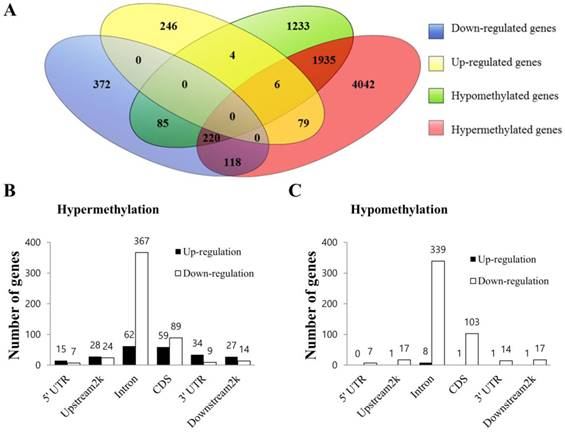
\includegraphics[width=0.8\textwidth]{journal-of-cancer_sample-result}}
	\caption{یک نمونه نمودار خلاصه برای نمایش نوآوری در نتایج
		%\cite{kim2016integrated}
	}
	\label{fig:sampleDiagram}
\end{figure}\\
طبیعتاً به صلاحدید نگارنده، شکل‌ها و نمودار‌ها می توانند در بخش های مختلف، خصوصا فصل
\ref{chap:results}
مورد استفاده قرار گیرند.

\subsection{تعریف واژه‌ها (اختیاری)}
در این قسمت محقق باید واژه‌هایی را که ممکن است برای خواننده آشنا نباشد، تعریف کند.

\subsection{خلاصه فصل‌ها}
در آخرین قسمتِ فصل اول پایان‌نامه، خلاصه‌ای اشاره‌وار از فصل‌های آتی آورده می‌شود تا خواننده بتواند تصویری واضح از دیگر قسمت‌های پایان‌نامه در ذهن خود ترسیم کند.

\section{جمع‌بندی}
در این فصل به دو مقولهٔ نحوه استفاده از قالب \پ دانشگاه تهران و نیز ویژگی‌هایی که محتویات فصل اول پایان‌نامه (یعنی مقدمه) باید داشته باشند، پرداخته شد. با توجه به اینکه این راهنما نحوه استفاده از قالب را شرح داده، ملزومات محتوایی هر فصل پایان‌نامه را توضیح می‌دهد و در پیوست‌ها نیز نحوهٔ کار با لاتک را یادآوری خواهد کرد، بنابراین مطالعهٔ کامل آن مقداری وقت شما را خواهد گرفت؛ اما مطمئن باشید از اتلاف وقت شما در ادامه کارتان تا حد زیادی جلوگیری خواهد کرد. در نوشتن متن حاضر سعی شده است علاوه بر ایجاد یک قالب لاتک برای پایان‌نامه‌های دانشگاه تهران، نکات محتوایی هر فصل نیز گوشزد گردد. طبیعتاً برای نگارش پایان‌نامهٔ خود می‌بایست مطالب تمام فصل‌ها را خودتان بازنویسی کنید.

در ادامهٔ این راهنما، تنها فصل‌هایی که یک پایان‌نامه باید داشته باشد و نیز خصوصیات یا ساختاری که محتویات هر فصل باید از آنها برخوردار باشد%
\footnote{از روی فایل «تمپلیت نگارش و تدوین پایان‌نامه \cite{UTThesisGuide}»}،
آورده می‌شوند. نهایتاً  در پیوست‌ها، مطالبی در باب یادآوری دستورات لاتک، نحوه نوشتن فرمول‌ها، تعاریف، قضایا، مثال‌ها، درج تصاویر، نمودارها، جداول و الگوریتم‌ها و نیز مدیریت مراجع، آمده است.

همچنین توصیه اکید دارم که رفع خطاهایی که احتمالاً با آنها مواجه می‌شوید را به آخر موکول نفرمایید و به محض برخورد با خطا، آن را اشکال‌زدایی و برطرف نمائید.		% فصل اول: مقدمه
% !TeX root=main.tex
\chapter{مروری بر مطالعات انجام شده}
%\thispagestyle{empty} 
\section{مقدمه}
هدف از اين فصل که با عنوان‌های  «مروری بر ادبیات موضوع%
\LTRfootnote{Literature Review}»،
«مروری بر منابع» و يا «مروری بر پیشینه تحقیق%
\LTRfootnote{Background Research}»
معرفی می‌شود، بررسی و طبقه‌بندی یافته‌های تحقیقات دیگر محققان در سطح دنیا و تعیین و شناسایی خلأهای تحقیقاتی است. آنچه را که تحقیق شما به دانش موجود اضافه می‌کند، مشخص کنید. طرح پیشینه تحقیق%
\LTRfootnote{Background Information}
یک مرور محققانه است و تا آنجا باید پیش برود که پیش‌زمینهٔ تاریخی مناسبی از تحقیق را بیان کند و جایگاه تحقیق فعلی را در میان آثار پیشین نشان دهد. برای این منظور منابع مرتبط با تحقیق را بررسی کنید، البته نه آنچنان گسترده که کل پیشینه تاریخی بحث را در برگیرد. برای نوشتن این بخش:
\begin{itemize}
	\item
	دانستنی‌های موجود و پیش‌زمینهٔ تاریخی و وضعیت کنونی موضوع را چنان بیان کنید که خواننده بدون مراجعه به منابع پیشین، نتایج حاصل از مطالعات قبلی را درک و ارزیابی کند.
	\item
	نشان دهید که بر موضوع احاطه دارید. پرسش تحقیق را همراه بحث و جدل‌ها و مسائل مطرح شده بیان کنید و مهم‌ترین تحقیق‌های انجام شده در این زمینه را معرفی نمائید.
	\item
	ابتدا مطالب عمومی‌تر و سپس پژوهش‌های مشابه با کار خود را معرفی کرده و نشان دهید که تحقیق شما از چه جنبه‌ای با کار دیگران تشابه یا تفاوت دارد.
	\item
	اگر کارهای قبلی را خلاصه کرده‌اید، از پرداختن به جزئیات غیرضروری بپرهیزید. در عوض، بر یافته‌ها و مسائل روش‌شناختی مرتبط و نتایج اصلی تأکید کنید و اگر بررسی‌ها و منابع مروری عمومی دربارهٔ موضوع موجود است، خواننده را به آنها ارجاع دهید.
\end{itemize}

\section{تعاریف، اصول و مبانی نظری}
این قسمت ارائهٔ خلاصه‌ای از دانش کلاسیک موضوع است. این بخش الزامی نیست و بستگی به نظر استاد راهنما دارد.

\section{مروری بر ادبیات موضوع}
در این قسمت باید به کارهای مشابه دیگران در گذشته اشاره کرد و وزن بیشتر این قسمت بهتر است به مقالات ژورنالی سال‌های اخیر (۲ تا ۳ سال) تخصیص داده شود. به نتایج کارهای دیگران با ذکر دقیق مراجع باید اشاره شده و جایگاه و تفاوت تحقیق شما نیز با کارهای دیگران مشخص شود. استفاده از مقالات ژورنال‌های معتبر در دو یا سه سال اخیر، می‌تواند به اعتبار کار شما بیافزاید.

\section{نتیجه‌گیری}
‌در نتیجه‌گیری آخر این فصل، با توجه به بررسی انجام شده بر روی مراجع تحقيق، بخش‌های قابل گسترش و تحقیق در آن حیطه و چشم‌اندازهای تحقیق مورد بررسی قرار می‌گیرند.	در برخی از تحقیقات، نتیجه نهایی فصل روش تحقیق، ارائهٔ یک چارچوب کار تحقیقی 
\lr{(research framework)}
است.		% فصول دوم: مروری بر مطالعات انجام شده
% !TeX root=main.tex
\chapter{روش تحقیق}
%\thispagestyle{empty} 
\section{مقدمه} 
این فصل، محل شرح كامل روش تحقيق است و بسته به نوع روش تحقيق و با نظر استاد راهنما می‌تواند «مواد و روش‌ها%
\LTRfootnote{Materials and Methods}»
نیز نام بگیرد. اين فصل حدود ۱۵ صفحه است.

\section{محتوا (نام‌گذاری بر اساس روش تحقیق و مسأله مورد مطالعه)}
\subsection{علت انتخاب روش}
دلیل یا دلایل انتخاب روش تحقیق را تشریح می‌کند.

\subsection{تشریح کامل روش تحقیق}
برای اینکه پایان‌نامه دارای ارزش علمی باشد، باید قابل تکرار باشد و داوران و خوانندگان از امکان تکرارپذیر بودن کار شما مطمئن شوند. شما باید چگونگی تکرار آزمایش به وسیله دیگران را در این قسمت فراهم کنید. تکرارپذیری آزمایشات و روش شما، برابر با میزان پتانسیل تکرار نتایجِ برابر یا نزدیک به آن است. در زير به تعدادی از روش‌های تحقیق اشاره شده است:
\begin{itemize}
	\item \textbf{روش تحقیق آزمایشگاهی}\\
	توصیف كامل برنامهٔ آزمایشگاهی شامل مواد مصرفی و نحوهٔ ساخت نمونه‌ها، شرح آزمایش‌ها شامل نحوه تنظیم و آماده‌سازی آزمایش‌ها و دستگاه‌های مورد استفاده، دقت و نحوهٔ كالیبره كردن، شرح دستگاه ساخته شده (در صورت ساخت) و ارائهٔ روش اعتبارسنجی.
	
	\item \textbf{روش تحقیق آماری}\\
	توصیف ابزارهای گردآوری اطلاعات کمی و کیفی، اندازهٔ نمونه‌ها، روش نمونه‌برداری، تشریح مبانی روش آماری و ارائهٔ روش اعتبارسنجی.
	
	\item \textbf{روش تحقیق نرم‌افزارنویسی}\\
	توصیف کامل برنامه‌نویسی، مبانی برنامه و ارائهٔ روش اعتبارسنجی.
	
	\item \textbf{روش تحقیق مطالعهٔ موردی}\\
	توصیف کامل محل و موضوع مطالعه، علت انتخاب مورد و پارامترهایی که تحت ارزیابی قرار داده می‌شوند و ارائهٔ روش اعتبارسنجی.

	\item \textbf{روش تحقیق تحلیلی یا مدل‌سازی}\\
	توصیف كامل مبانی یا اصول تحلیل یا مدل و ارائهٔ روش اعتبارسنجی آن. در ارائه مدل ریاضی معمولاً نیاز است اندیس‌ها، پارامترها، متغیرهای تصمیم و فرمول‌های مدل، به صورت سیستماتیک ارائه شوند. پیشنهاد می‌گردد برای نمایش اندیس‌ها، پارامترها و متغیرهای تصمیم از سه جدول به صورت زیر استفاده گردد:
	\begin{table}[ht]
		\caption{اندیس‌های به کار رفته در مدل ریاضی}
		\label{tab:modelIndices}
		\centering
		\onehalfspacing
		\begin{tabularx}{0.9\textwidth}{|r|X|}
			\hline
			$I, J$	& بیماران \\
			\hline
			$k$		& مرحله زمان‌بندی (بستری، اتاق عمل، ریکاوری) \\
			\hline
			$L_k$	& ماشین (تخت یا اتاق عمل) در مرحله $k$ \\
			\hline
			$n$		&  جراح \\
			\hline
		\end{tabularx}
	\end{table}
	
	\begin{table}[ht]
		\caption{پارامترهای مدل ریاضی}
		\label{tab:modelParameters}
		\centering
		\onehalfspacing
		\begin{tabularx}{0.9\textwidth}{|r|X|}
			\hline
			$t_{ik}$			& زمان خدمت‌دهی به بیمار در مرحله $k$ام \\
			\hline
			$\tilde{t}_{ik}$	& زمان فاری خدمت‌دهی به بیمار در محله $k$ام \\
			\hline
			$t_{ik}^p$			& مقدار بدبینانه (حداکثر) برای زمان خدمت‌دهی به بیمار در مرحله $k$ام \\
			\hline
			$t_{ik}^m$			& محتمل‌ترین مقدار برای زمان خدمت‌دهی به بیمار در مرحله $k$ام \\
			\hline
			$t_{ik}^o$			& مقدار خوشبینانه (حداقل) برای زمان خدمت‌دهی به بیمار در مرحله $k$ام \\
			\hline
		\end{tabularx}
	\end{table}
	
	\begin{table}[ht]
		\caption{متغیرهای مدل ریاضی}
		\label{tab:modelVariables}
		\centering
		\onehalfspacing
		\begin{tabularx}{0.9\textwidth}{|r|X|}
			\hline
			$X_{ild_{k}}$	& متغیر صفر-یک تخصیص بیمار به تخت/اتاق عمل\\
			\hline
			$S_{ild_{k}}$	& زمان شروع خدمت‌دهی به بیمار \\
			\hline
			$Y_{ijkl_{k}}$	& متغیر صفر-یک توالی بیماران \\
			\hline
			$V_{ni}$		& متغیر صفر-یک تخصیص جراح به بیمار‍‍ \\
			\hline
		\end{tabularx}
	\end{table}
	
	\item \textbf{روش تحقیق میدانی}\\
	چگونگی دستیابی به داده‌ها در میدان عمل و نحوه برداشت از پاسخ‌های دریافتی.
\end{itemize}		% فصل سوم: روش تحقیق
% !TeX root=../main.tex
\chapter{نتایج}
%\thispagestyle{empty} 
\label{chap:results}
\section{مقدمه} 
ارائهٔ داده‌ها، نتایج، تحلیل و تفسیر اولیهٔ آنها در این فصل ارائه می‌شود. در ارائهٔ نتایج با توجه به راهنمای کلی نگارش فصل‌ها، تا حد امکان، ترکیبی از نمودار و جدول استفاده شود. با توجه به حجم و ماهیت تحقیق و با صلاحدید استاد راهنما، این فصل می‌تواند تحت عنوانی دیگر بیاید. در صورتی که حجم داده‌ها زیاد باشد، بهتر است به صورت نمودار یا در قالب ضمیمه ارائه نشده و فقط نمونه‌ها در متن آورده شود. در این فصل باید به سوالات تحقیق، عطف به یافته‌های محقق، پاسخ داده شود. اگر تحقیق دارای آزمون فرض باشد، پذیرش یا عدم پذیرش فرضیه‌ها در این فصل گزارش می‌شود. این فصل حدود ۴۰ صفحه است.

\section{محتوا}
در این بخش به سوالات تحقیق، بر اساس داده‌ها و یافته‌های محقق، پاسخ داده می‌شود. داده‌ها با فرمت مناسبی ارائه می‌شوند؛ مدل (ها) اجرا شده و نتیجه آن مشخص می‌شود.

\section{اعتبارسنجی}
از طریق مقایسهٔ نتایج با نتایج کارهای دیگران، استفاده از روش‌های تحلیل پایائی
\lr{(reliability)}
و اعتبار
\lr{(validity)}،
نظرگیری از خبرگان
\lr{(expert judgment or feedback)}
و یا
\lr{triangulation}
انجام می‌شود.
		% فصل چهارم: نتایج
% !TeX root=main.tex
\chapter{بحث و نتیجه‌گیری}
%\thispagestyle{empty} 
\section{مقدمه}
تاکنون شما در پایان‌نامه‌ای که مشغول نوشتن آن هستید، پاسخ چهار سؤال را داده‌اید:
\begin{itemize}
	\item
	چرا تحقیق را انجام دادید؟ (مقدمه)
	\item
	دیگران در این زمینه‌ چه کارهایی کرده‌اند و تمایز کار شما با آنها؟ (مرور ادبیات)
	\item
	چگونه تحقیق را انجام دادید؟ (روش‌ها)
	\item
	چه از تحقیق به دست آوردید؟ (یافته‌ها)
\end{itemize}
حال زمان آن فرا رسیده که با توجه به تمامی مطالب ذکر شده، در نهایت به سؤال آخر پاسخ دهید:
\begin{itemize}
	\item
	چه برداشتی از یافته‌های تحقیق کردید؟ (نتیجه‌گیری)
\end{itemize}
در واقع در این بخش، هدف، پاسخ به این سوال است که چه برداشتی از یافته‌ها کردید و این یافته‌ها چه فایده‌ای دارند؟

نتیجه‌گیری مختصری بنویسید. ارائهٔ داده‌ها، نتایج و یافته‌ها در فصل چهارم ارائه می‌شود. در این فصل تفاوت، تضاد یا تطابق بین نتایج تحقیق با نتایج دیگر محققان باید ذکر شود.
\emph{تفسیر و تحلیل نتایج نباید بر اساس حدس و گمان باشد}،
بلکه باید
\textbf{برمبنای نتایج عملی استخراج‌شده}
از تحقیق و یا
\textbf{استناد به تحقیقات دیگران}
باشد.
با توجه به حجم و ماهیت تحقیق و با صلاحدید استاد راهنما، این فصل می‌تواند تحت عنوانی دیگر بیاید یا به دو فصل جداگانه با عناوین مناسب، تفکیک شود. اين فصل فقط باید به جمع‌بندی دست‌آوردهای فصل‌های سوم و چهارم محدود و از ذکر موارد جدید در آن خودداری شود. در عنوان این فصل، به جای کلمهٔ «تفسیر» می‌توان از واژگان «بحث» و «تحلیل» هم استفاده کرد. این فصل شاید مهم‌ترین فصل پایان‌نامه باشد.

در این فصل خلاصه‌ای از یافته‌های تحقیق جاری ارائه می‌شود. این فصل می‌تواند حاوی یک مقدمه، شامل مروری اجمالی بر مراحل انجام تحقیق باشد (حدود یک صفحه). مطالب پاراگراف‌بندی شود و هر پاراگراف به یک موضوع مستقل اختصاص یابد. فقط به ارائهٔ یافته‌ها و دست‌آوردها بسنده شود و
\emph{از تعمیم بی‌مورد نتایج خودداری شود.}
تا حد امکان از ارائهٔ 
\emph{جداول و نمودارها در این فصل اجتناب شود.}
از ارائهٔ 
\emph{عناوین کلی}
در حوزهٔ تحقیق و قسمت پيشنهاد تحقیقات آتی خودداری شود و کاملاً در چارچوب و زمينهٔ مربوط به تحقیق جاری باشد. این فصل حدود ۱۰-۱۵ صفحه است.

\section{محتوا}
به ترتیب شامل موارد زیر است:

\subsection{جمع‌بندی}
خلاصه‌ای از تمام یافته‌ها و دست‌آوردهای تحقیق جاری است.

\subsection{نوآوری}
این قسمت، نوآوری تحقیق را بر اساس یافته‌های آن تشریح می‌کند. که دارای دو بخش اصلی است:
\begin{enumerate}
	\item
	نوآوری تئوری، یعنی تمایز تئوریک کار با کارهای محققین قبلی.
	\item
	نوآوری عملی، یعنی توصیه‌های محقق به صنعت برای بهبود بخشیدن به کارها، بر اساس یافته‌های تحقیق.
\end{enumerate}

\subsection{پیشنهادها}
این بخش، عناوین و موضوعات پیشنهادی را برای تحقیقات آتی،
\emph{بیشتر در زمينهٔ مورد بحث در آينده}
ارائه می‌کند.

\subsection{محدودیت‌ها}
در اینجا انواع محدودیت‌های تحقیق تشریح می‌شوند؛ از جمله، محدودیت‌هایی که کنترل آن از عهده محقق خارج است، مانند انتخاب نوع یافته‌ها؛ و همچنین دیگر محدودیت‌هایی که کنترل آن در دست محقق است، مانند موضوع و محل تحقیق و ... . تأثیر این محدودیت‌ها بر یافته‌های تحقیق در این قسمت شرح داده می‌شوند.		% فصل پنجم: بحث و نتیجه‌گیری

% مراجع
% اگر از استیل‌های natbib استفاده می‌کنید باید دو خط را در فایل commands.tex تغییر دهید.
\pagestyle{empty}
{
\small
\onehalfspacing
\bibliographystyle{plain-fa} % or plainnat-fa for author-date
\bibliography{./tex/MyReferences}
}

\pagestyle{fancy}

% \appendix
% فصلهای پس از این قسمت به عنوان ضمیمه خواهند آمد.

% دستورات لازم برای تبدیل «فصل آ» به «پیوست آ» در فهرست مطالب
\addtocontents{toc}{
    \protect\renewcommand\protect\cftchappresnum{\appendixname~}%
    \protect\setlength{\cftchapnumwidth}{\mylenapp}}
    
% دستورات لازم برای شماره‌گذاری صفحات پیوست‌ها بشکل آ-۱ (فعلا با glossaries سازگار نیست)
% \let\Chapter\chapter
%\pretocmd{\chapter}{
%  \clearpage
%  \pagenumbering{arabic}
%  \renewcommand*{\thepage}{\rl{\thechapter-\arabic{page}}}}{}{}
%%%%%%%%%%%%%%%%%%%%%%%%%%%%%%%%%%%%%
        

% !TeX root=main.tex
%% دو سری دستور زیر باید در اولین فایل پیوست باشند. آنها را حذف نکنید!
% دستورات لازم برای تبدیل «فصل آ» به «پیوست آ» در فهرست مطالب
\addtocontents{toc}{
    \protect\renewcommand\protect\cftchappresnum{\appendixname~}%
    \protect\setlength{\cftchapnumwidth}{\mylenapp}}
    
\let\Chapter\chapter
% دستورات لازم برای شماره‌گذاری صفحات پیوست‌ها بشکل آ-۱
%\pretocmd{\chapter}{
%  \clearpage
%  \pagenumbering{arabic}
%  \renewcommand*{\thepage}{\rl{\thechapter-\arabic{page}}}}{}{}
%%%%%%%%%%%%%%%%%%%%%%%%%%%%%%%%%%%%%
    
\chapter{آشنایی سریع با برخی دستورات لاتک}
\label{app:latexIntro}
%\thispagestyle{empty}
در این فصل ویژگی‌های مهم و پرکاربرد زی‌پرشین و لاتک معرفی می‌شود. برای راهنمایی بیشتر و به‌کاربردن ویژگی‌های پیشرفته‌تر به راهنمای زی‌پرشین و راهنمای لاتک مراجعه کنید. برای آگاهی از دستورات لاتک که این خروجی را تولید کرده‌اند فایل \lr{appendix1.tex} را ملاحظه فرمایید.
\footnote{بیشتر مطالب این بخش از مثال 
\lr{xepersian\_example.tex}
گرفته شده‌اند که توسط آقای امیرمسعود پورموسی آماده شده است.}

\section{بندها و زیرنویس‌ها}
هر جایی از نوشتهٔ خود، اگر می‌خواهید به سر سطر بروید و یک بند (پاراگراف) تازه را آغاز کنید، باید یک خط را خالی بگذارید%
\footnote{یعنی دوبار باید کلید \lr{Enter} را بزنید.}
 مانند این:

حالا که یک بند تازه آغاز شده است، یک زیرنویس انگلیسی%
\LTRfootnote{English Footnote!}
 هم می‌نویسیم!
\section{فرمول‌های ریاضی}
\label{formula}

اینجا هم یک فرمول می‌آوریم که شماره دارد:
\begin{equation}\label{eq:yek}
A=\frac{c}{d}+\frac{q^2}{\sin(\omega t)+\Omega_{12}}
\end{equation}
در لاتک می‌توان به کمک فرمان 
\lr{\textbackslash label\{\}}
به هر فرمول یک نام نسبت داد. در فرمول بالا نام \lr{eq:yek} را برایش گذاشته‌ایم (پروندهٔ \lr{tex} همراه با این مثال را ببینید). این نام ما را قادر می‌کند که بعداً بتوانیم با فرمان
\lr{\textbackslash ref\{eq:yek\}}
به آن فرمول با شماره ارجاع دهیم. یعنی بنویسیم فرمول \ref{eq:yek}. 
لاتک خودش شمارهٔ این فرمول‌ها را مدیریت می‌کند.\footnote{یعنی اگر بعداً فرمولی قبل از این فرمول بنویسیم، خودبه‌خود شمارهٔ این فرمول و شمارهٔ ارجاع‌ها به این فرمول یکی زیاد می‌شود. دیگر نگران شماره‌گذاری فرمول‌های خود نباشید!} این هم یک فرمول که شماره ندارد:
$$A=|\vec{a}\times \vec{b}| + \sum_{n=0}^\infty C_{ij}$$

این هم عبارتی ریاضی مانند 
$\sqrt{a^2+b^2}$
 که بین متن می‌آید.
\subsection{یک زیربخش}
\label{zirbakhsh}

این زیربخش \ref{zirbakhsh} است؛ یعنی یک بخش درون بخش \ref{formula} است.
\subsubsection{یک زیرزیربخش}
این هم یک زیرزیربخش است. در لاتک می‌توانید بخش‌های تودرتو در نوشته‌تان تعریف کنید تا ساختار منطقی نوشته را به خوبی نشان دهید. می‌توانید به این بخش‌ها هم با شماره ارجاع دهید، مثلاً بخش فرمول‌های ریاضی شماره‌اش \ref{formula} است.
\section{نوشته‌های فارسی و انگلیسی مخلوط}
نوشتن یک کلمهٔ انگلیسی بین متن فارسی بدیهی است، مانند Example در این جمله.
نوشتن یک عبارت چندکلمه‌ای مانند
 \lr{More than one word} کمی پیچیده‌تر است.

اگر ناگهان تصمیم بگیرید که یک بند کاملاً انگلیسی را بنویسید، باید:
\begin{latin}
This is an English paragraph from left to right. You can write as much as you want in it.
\end{latin}
\section{افزودن تصویر به نوشته}
پروندهٔ تصویر دلخواه خود را در کنار پروندهٔ \lr{tex} قرار دهید. سپس به روش زیر تصویر را در نوشتهٔ خود بیاورید:
\begin{latin}
\begin{verbatim}
\includegraphics{YourImageFileName}
\end{verbatim}
\end{latin}
به تصویرها هم مانند فرمول‌ها و بخش‌ها می‌توان با شماره ارجاع داد. مثلاً تصویر \ref{fig:shir} یک شیر علاقه‌مند به لاتک را در حال دویدن نشان می‌دهد. برای جزئیات بیشتر دربارهٔ روش گذاشتن تصویرها در نوشته باید راهنماهای لاتک را بخوانید.
\begin{figure}[ht]
\centerline{
\includegraphics[width=5cm]{lion}}
\caption{در این تصویر یک شیر علاقه‌مند به لاتک را در حال دویدن می‌بینید.}
\label{fig:shir}
\end{figure}

به تصویرها هم مانند فرمول‌ها و بخش‌ها می‌توان با شماره ارجاع داد. مثلاً تصویر بالا شماره‌اش \ref{fig:shir} است. برای جزئیات بیشتر دربارهٔ روش گذاشتن تصویرها در نوشته باید راهنماهای لاتک را بخوانید.

\section{محیط‌های شمارش و نکات}
برای فهرست‌کردن چندمورد، اگر ترتیب برایمان مهم نباشد:
\begin{itemize}
\item مورد یکم
\item مورد دوم
\item مورد سوم
\end{itemize}
و اگر ترتیب برایمان مهم باشد:
\begin{enumerate}
\item مورد یکم
\item مورد دوم
\item مورد سوم
\end{enumerate}
می‌توان موردهای تودرتو داشت:
\begin{enumerate}
\item مورد ۱
\item مورد ۲
\begin{enumerate}
\item مورد ۱ از ۲
\item مورد ۲ از ۲
\item مورد ۳ از ۲
\end{enumerate}
\item مورد ۳
\end{enumerate}
شماره‌گذاری این موردها را هم لاتک انجام می‌دهد.

\section{تعریف و قضیه}
برای ذکر تعریف، قضیه و مثال مثالهای ذیل را ببینید.
\begin{definition}
مجموعه همه ارزیابی‌های  (پیوسته)  روی $(X,\tau)$، دامنه توانی احتمالی
\index{دامنه توانی احتمالی}
$ X $
نامیده می‌شود.
\end{definition}
\begin{theorem}[باناخ-آلااغلو]
\index{قضیه باناخ-آلااغلو}
اگر $ V $ یک همسایگی $ 0 $ در فضای برداری 
\index{فضای!برداری}
 توپولوژیکی $ X $ باشد و 
\begin{equation}\label{eq1}
K=\left\lbrace \Lambda \in X^{*}:|\Lambda x|\leqslant 1 ; \ \forall x\in V\right\rbrace,
\end{equation}
آنگاه $ K $،  ضعیف*-فشرده است که در آن، $ X^{*} $ دوگان
\index{فضای!دوگان}
 فضای برداری توپولوژیکی $ X $ است به ‌طوری که عناصر آن،  تابعی‌های 
خطی پیوسته
\index{تابعی خطی پیوسته}
 روی $X$ هستند.
\end{theorem}
تساوی \eqref{eq1} یکی از مهم‌ترین تساوی‌ها در آنالیز تابعی است که در ادامه، به وفور از آن استفاده می‌شود.
\begin{example}
برای هر فضای مرتب، گردایه 
$$U:=\left\lbrace U\in O: U=\uparrow U\right\rbrace $$
از مجموعه‌های بالایی باز، یک توپولوژی تعریف می‌کند که از توپولوژی اصلی، درشت‌تر  است.
\end{example}
حال تساوی 
\begin{equation}\label{eq2}
\sum_{n=1}^{+\infty} 3^{n}x+7x=\int_{1}^{n}8nx+\exp{(2nx)}
\end{equation}
را در نظر بگیرید. با مقایسه تساوی \eqref{eq2} با تساوی \eqref{eq1} می‌توان نتیجه گرفت که ...


\section{چگونگی نوشتن و ارجاع به مراجع}
\label{Sec:Ref}


در لاتک به راحتی می‌توان مراجع خود را نوشت و به آنها ارجاع داد. به عنوان مثال برای معرفی کتاب گنزالس \cite{Gonzalez02book} به عنوان یک مرجع می‌توان آنرا به صورت زیر معرفی نمود:

\singlespacing
\begin{LTR}
\begin{verbatim}
\bibitem{Gonzalez02book}
Gonzalez, R.C., and Woods, R.E. {\em Digital Image Processing}, 3rd ed..
Prentice-Hall, Inc., Upper Saddle River, NJ, USA, 2006.
\end{verbatim}
\end{LTR}
\doublespacing

در دستورات فوق \lr{Gonzalez02book}  برچسبی است که به این مرجع داده شده است و با استفاده از دستور 
\verb!\cite{Gonzalez02book}!
می‌توان به آن ارجاع داد؛ بدون این که شماره‌اش را در فهرست مراجع‌مان بدانیم.

اگر این اولین مرجع ما باشد در قسمت مراجع به صورت زیر خواهد آمد:\\
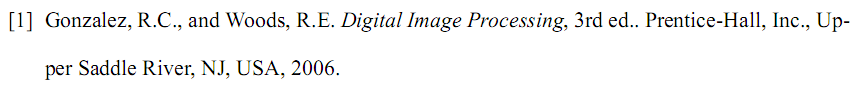
\includegraphics[width=\textwidth]{gonzalez.png}

این شیوهٔ تعریف مراجع بسیار ابتدایی است و اگر فرمت مراجع، ترتیب یا تعداد آنها را خواسته باشید تغییر دهید، به عنوان مثال ابتدا حرف اول نام نویسنده بیاید و سپس نام خانوادگی، باید همه کارها را به صورت دستی انجام دهید!
چون در یک \پ یا مقاله باید کنترل کاملی بر مراجع خود داشته باشید و به راحتی بتوانید قالب مراجع را عوض کنید، بنابراین می‌بایست از \lr{Bib\TeX} استفاده کنید که درپیوست  \ref{app:refMan} به  آن پرداخته خواهد شد.
		% پیوست اول: آشنایی مقدماتی با لاتک
% !TeX root=../main.tex

\chapter{‌جدول، نمودار و الگوریتم در لاتک}
\label{app:latex:more}
%\thispagestyle{empty}

در این بخش نمونه مثالهایی از جدول، شکل، نمودار، الگوریتم و معادلات ریاضی را در لاتک خواهیم دید.
دقت کنید که در پایان‌نامه‌ها و مقالات، باید قاعدهٔ «ارجاع به جلو%
\LTRfootnote{Forward Referencing}»
رعایت شود؛ یعنی ابتدا در متن به شمارهٔ شکل، جدول یا معادله اشاره شود و بعد از آن (زیر آن) خود شکل، جدول یا معادله رسم شود. (توضیحات بیشتر در قسمت
\ref{sec:floatObjs}).

\section{جدول}
دستور اصلی برای رسم جدول در لاتک 
\verb|tabular|
می‌باشد که جدول
\eqref{tab:motionModels}
با استفاده از آن کشیده شده است؛ در
\verb|tabular|
عرض جدول برابر با مجموع عرض ستون‌ها و حداکثر مساوی عرض متن است.
\begin{table}[ht]
\caption{مدلهای تبدیل.}
\label{tab:motionModels}
\centering
\onehalfspacing
\begin{tabular}{|r|c|l|r|}
	\hline نام مدل & درجه آزادی & تبدیل مختصات & توضیح \\ 
	\hline انتقالی & ۲ & $\begin{aligned} x'=x+t_x \\ y'=y+t_y \end{aligned}$  &  انتقال دوبعدی\\ 
	\hline اقلیدسی & ۳ & $\begin{aligned} x'=x\cos\theta - y\sin\theta+t_x \\ y'=x\sin\theta+y\cos\theta+t_y \end{aligned}$  &  انتقالی+دوران \\ 
	\hline 
\end{tabular} 
\end{table}

برای اینکه عرض جدول قابل کنترل باشد، باید از دستورات
\verb|tabularx|،
\verb|tabulary| یا
\verb|tabu|
استفاده کرد که راهنمای آنها در اینترنت وجود دارد.
مثلاً جدول
\ref{tab:motionModelsCont}
با
\verb|tabularx|
رسم شده که عرض جدول در آن ثابت بوده و ستون‌های از نوع
\verb|X|
عرض خالی جدول را پر می‌کنند.
\begin{table}[ht]
	\caption{مدلهای تبدیل دیگر.}
	\label{tab:motionModelsCont}
	\centering
	\onehalfspacing
	\begin{tabularx}{\textwidth}{|r|c|l|X|}
		\hline نام مدل & درجه آزادی & تبدیل مختصات & توضیح \\ 
		\hline مشابهت & ۴ & $\begin{aligned} x'=sx\cos\theta - sy\sin\theta+t_x \\ y'=sx\sin\theta+sy\cos\theta+t_y  \end{aligned}$  & اقلیدسی+تغییرمقیاس \\ 		
		\hline آفین & ۶ & $\begin{aligned} x'=a_{11}x+a_{12}y+t_x \\ y'=a_{21}x+a_{22}y+t_y \end{aligned}$  & مشابهت+اریب‌شدگی \\
		\hline
	\end{tabularx}
\end{table}

\section{معادلات ریاضی و ماتریس‌ها}
تقریباً هر آنچه دانشجویان برای نوشتن فرمول‌های ریاضی لازم دارند، در کتاب 
\lr{mathmode}
آمده است. کافیست در خط فرمان، دستور زیر را وارد کنید:
\begin{latin}
	\texttt{texdoc mathmode}
\end{latin}
متن زیر شامل انواعی از اشیاء ریاضی است که با ملاحظه کدش می‌توانید با دستورات آن آشنا شوید.\\
شناخته‌شده‌ترین روش تخمین ماتریس هوموگرافی الگوریتم تبدیل خطی مستقیم (\lr{DLT\LTRfootnote{Direct Linear Transform}}) است.  فرض کنید چهار زوج نقطهٔ متناظر در دو تصویر در دست هستند،  $\mathbf{x}_i\leftrightarrow\mathbf{x}'_i$   و تبدیل با رابطهٔ
  $\mathbf{x}'_i = H\mathbf{x}_i$
  نشان داده می‌شود که در آن:
\[\mathbf{x}'_i=(x'_i,y'_i,w'_i)^\top  \]
و
\[ H=\left[
\begin{array}{ccc}
h_1 & h_2 & h_3 \\ 
h_4 & h_5 & h_6 \\ 
h_7 & h_8 & h_9
\end{array} 
\right]\]
رابطه زیر را برای الگوریتم  \eqref{alg:DLT} لازم داریم.
\begin{equation}
\label{eq:DLT_Ah}
\left[
\begin{array}{ccc}
	0^\top & -w'_i\mathbf{x}_i^\top & y'_i\mathbf{x}_i^\top \\ 
	w'_i\mathbf{x}_i & 0^\top & -x'_i\mathbf{x}_i^\top \\ 
	- y'_i\mathbf{x}_i^\top & x'_i\mathbf{x}_i^\top & 0^\top
\end{array} 
\right]
\left(
\begin{array}{c}
	\mathbf{h}^1 \\ 
	\mathbf{h}^2 \\ 
	\mathbf{h}^3
\end{array} 
\right)=0
\end{equation}

\section{الگوریتم}

\subsection{الگوریتم ساده با دستورهای فارسی}
با مفروضات فوق، الگوریتم \lr{DLT} به صورت نشان داده شده در الگوریتم \eqref{alg:DLT}  خواهد بود.
\begin{algorithm}[ht]
\onehalfspacing
\caption{الگوریتم \lr{DLT} برای تخمین ماتریس هوموگرافی.} \label{alg:DLT}
\begin{algorithmic}[1]
\REQUIRE $n\geq4$ زوج نقطهٔ متناظر در دو تصویر 
${\mathbf{x}_i\leftrightarrow\mathbf{x}'_i}$،\\
\ENSURE ماتریس هوموگرافی $H$ به نحوی‌که: 
$\mathbf{x}'_i = H \mathbf{x}_i$.
  \STATE برای هر زوج نقطهٔ متناظر
$\mathbf{x}_i\leftrightarrow\mathbf{x}'_i$ 
ماتریس $\mathbf{A}_i$ را با استفاده از رابطهٔ \ref{eq:DLT_Ah} محاسبه کنید.
  \STATE ماتریس‌های ۹ ستونی  $\mathbf{A}_i$ را در قالب یک ماتریس $\mathbf{A}$ ۹ ستونی ترکیب کنید. 
  \STATE تجزیهٔ مقادیر منفرد \lr{(SVD)}  ماتریس $\mathbf{A}$ را بدست آورید. بردار واحد متناظر با کمترین مقدار منفرد جواب $\mathbf{h}$ خواهد بود.
  \STATE  ماتریس هوموگرافی $H$ با تغییر شکل $\mathbf{h}$ حاصل خواهد شد.
\end{algorithmic}
\end{algorithm}

\subsection{الگوریتم پیچیده و تودرتو با دستورهای فارسی}
الگوریتم \ref{alg:simulation-random}، یک الگوریتم ترکیبی و تودرتو است که با کمک دستورهای بسته‌ی \lr{algorithmic} نوشته شده است.

\begin{algorithm}[p]
    \onehalfspacing
    \caption{الگوریتم اجرای برنامه‌ی شبیه‌سازی}
    \label{alg:simulation-random}
    \begin{algorithmic}[1]
        \REQUIRE زمان $t_{max}$ به عنوان زمان لازم برای انجام شبیه سازی،\\
        \REQUIRE  گراف شبکه برای شبیه سازی،
        \ENSURE جدول تغییرات گراف از لحظه‌ی ۰ تا t.
        \FOR {تمام لحظات در بازه‌ی ۰ تا $t_{max}$}
            \FOR {تمام پیوند‌ها}
                \STATE محاسبه‌ی ضریب و نرخ انتقال پیوند
                \STATE محاسبه‌ی کیفیت و نرخ یادگیری
            \ENDFOR
            \FOR {تمام گره‌ها}
                \STATE محاسبه‌ی نرخ انتقال گره
                \STATE محاسبه‌ی وضعیت جدید
            \ENDFOR
            \IF {تغییرات از مقدار $\delta$ کمتر است}
                \STATE شکستن حلقه
                \COMMENT{این شرط برای پایان قبل از رسیدن به محدودیت زمانی است، اگر تغییرات کمتر از $\delta$ باشد}
            \ELSIF {زمان اجرای برنامه بیش از حد طول کشیده \AND $t>100$}
                \STATE شکستن حلقه
            \ENDIF
        \ENDFOR
        \PRINT {زمان اجرای برنامه}
        \RETURN {ماتریس تغییرات زمانی}
    \end{algorithmic}
\end{algorithm}

\subsection{الگوریتم با دستورهای لاتین}
الگوریتم \ref{alg:RANSAC} یک الگوریتم با دستورهای لاتین است.

\begin{algorithm}[ht]
\onehalfspacing
\caption{الگوریتم \lr{RANSAC} برای تخمین ماتریس هوموگرافی.} \label{alg:RANSAC}
\begin{latin}
\begin{algorithmic}[1]
\REQUIRE $n\geq4$ putative correspondences, number of estimations, $N$, distance threshold $T_{dist}$.\\
\ENSURE Set of inliers and Homography matrix $H$.
\FOR{$k = 1$ to $N$}
  \STATE Randomly choose 4 correspondence,
  \STATE Check whether these points are colinear, if so, redo the above step
  \STATE Compute the homography $H_{curr}$ by DLT algorithm from the 4 points pairs,
  \STATE $\ldots$ % الگوریتم کامل نیست
  \ENDFOR
  \STATE Refinement: re-estimate H from all the inliers using the DLT algorithm.
\end{algorithmic}
\end{latin}
\end{algorithm}

\section{کد}
درج کد به زبان‌های مختلف به سادگی امکان‌پذیر است. برنامه
\ref{code:matlabEx}
یک قطعه کد
\lr{MATLAB}
را نشان می‌دهد.
\begin{figure}[ht]
	\begin{LTR}
        \singlespacing
		\lstinputlisting[language=MATLAB, caption={نمونه کد \lr{MATLAB}}, label={code:matlabEx}]{MatlabExample.m}
        % \doublespacing
	\end{LTR}
\end{figure}

\section{تصویر}
نمونهٔ یک تصویر را در فصل قبل دیدیم. دو تصویر شیر کنار هم را نیز در شکل
\ref{fig:twoLion}
مشاهده می‌کنید.
\begin{figure}[ht]
\centering 
\subfloat[شیر ۱]{ \label{fig:twolion:one}

\includegraphics[width=0.3\textwidth]{lion}}
%\hspace{2mm}
\subfloat[شیر ۲]{ \label{fig:twolion:two}

\includegraphics[width=0.3\textwidth]{lion}}%
\caption{دو شیر}
\label{fig:twoLion} %% label for entire figure
\end{figure}

\section{نمودار}
لاتک بسته‌هایی با قابلیت‌های زیاد برای رسم انواع مختلف نمودارها دارد. مانند بسته‌های \lr{Tikz} و  \lr{PSTricks}. توضیح اینها فراتر از این پیوست کوچک است.%
\footnote{
مثال‌هایی از بکارگیری بسته
\lr{Tikz}
را می‌توانید در
\url{http://www.texample.net/tikz/examples/}
ببینید. توصیه می‌شود دانشجویانی که قصد درج اشکالی مانند گراف را در سند خود دارند، مثالهایی از سایت مذکور را ملاحظه فرمایند.
}
یک نمودار رسم شده با بسته‌ی 
\lr{TikZ}
 در شکل 
\ref{fig:parabola}
نشان داده شده است.
\begin{figure}[t]
\centering
\begin{tikzpicture}[scale=2.5]
  \shade[top color=blue,bottom color=gray!50] 
      (0,0) parabola (1.5,2.25) |- (0,0);
  \draw (1.05cm,2pt) node[above] 
      {$\displaystyle\int_0^{3/2} \!\!x^2\mathrm{d}x$};

  \draw[style=help lines] (0,0) grid (3.9,3.9)
       [step=0.25cm]      (1,2) grid +(1,1);

  \draw[->] (-0.2,0) -- (4,0) node[right] {$x$};
  \draw[->] (0,-0.2) -- (0,4) node[above] {$f(x)$};

  \foreach \x/\xtext in {1/1, 1.5/1\frac{1}{2}, 2/2, 3/3}
    \draw[shift={(\x,0)}] (0pt,2pt) -- (0pt,-2pt) node[below] {$\xtext$};

  \foreach \y/\ytext in {1/1, 2/2, 2.25/2\frac{1}{4}, 3/3}
    \draw[shift={(0,\y)}] (2pt,0pt) -- (-2pt,0pt) node[left] {$\ytext$};

  \draw (-.5,.25) parabola bend (0,0) (2,4) node[below right] {$x^2$};
\end{tikzpicture}
\caption{یک نمودار زیبا با ارقام فارسی و قابلیت بزرگ‌نمایی بسیار، بدون از دست دادن کیفیت.}
\label{fig:parabola}
\end{figure}

\section{نحوه قرارگیری اشیای شناور}
\label{sec:floatObjs}
شکل‌ها، جداول و الگوریتم‌ها در لاتک اشیای شناور محسوب می‌شوند؛ یعنی خود لاتک تصمیم می‌گیرد آنها را در کجای صفحه ترسیم کند تا زیباتر باشد. اما می‌توان به لاتک توصیه کرد که آن را در قسمت خاصی از صفحه رسم کند. برای اینکه قاعدهٔ «ارجاع به جلو» رعایت شود باید فقط از پرچم
\verb|[ht]|
استفاده کرد، که می‌گوید اگر جا شد شکل را دقیقاً در همین مکان و در غیراینصورت در بالای صفحه بعد رسم کن.
بنابراین دستورات درج تصویر، جدول و الگوریتم به صورت زیر باید باشند:

\begin{latin}
\begin{verbatim}
	\begin{figure/table/algorithm}[ht]
		...
	\end{figure/table/algorithm}
\end{verbatim}
\end{latin}
		% پیوست دوم: جدول، نمودار و الگوریتم در لاتک
% !TeX root=../main.tex
\chapter{مراجع، واژه‌نامه و حاشیه‌نویسی}
\label{app:refMan}
%\thispagestyle{empty}

\section{مراجع و نقل‌قول‌ها}
\label{sec:refUsage}
منابعِ پایان‌نامه، پایه و اساس تحقیق شما به حساب می‌آیند و ضرورت انجام مطالعه و روش‌های به کار رفته در بسیاری از قسمت‌های آن، به کمک منابع صورت می‌گیرد. در استفاده از مراجع علمی در پایان‌نامه، باید سعی کنید بیشتر از
\textbf{منابع چاپ‌شده و مهم}
استفاده کنید و
\emph{ارجاع به داده‌های چاپ نشده، خلاصه‌ها و پایان‌نامه‌ها، سبب به‌هم‌خوردگی و کاهش اعتبار قسمت ارجاع منابع می‌شود.}
استفاده از منابع و نقل قول‌هایی به تحقیق شما ارزش می‌دهند که
\textbf{در راستای هدف تحقیق بوده و به آن اعتبار ببخشند.}
برخی از دانش‌جویان تصوّر می‌کنند که کثرت نقل‌قول‌ها و ارجاعات زیاد، مهم‌ترین معیار علمی شدن پایان‌نامه است؛ حال آنکه استناد به تعداد کثیری از منابع بدون مطالعه دقیق آنها و استفادهٔ مستقیم در پایان‌نامه، می‌تواند نشان‌دهندهٔ عدم احساس امنیت نویسنده باشد!

دو روش برای استفاده از نتایج، جملات، داده‌ها و روش‌های دیگران وجود دارد. یکی نقل‌قول مستقیم و دقیق است و دیگری استفاده غیرمستقیم در متن مقاله، که در ادامه به قواعد این دو نوع نقل‌قول و ارجاع‌دهی اشاره می‌کنیم:
\begin{description}
	\item[نقل‌قول مستقیم:]
	نقل‌قول مستقیم باید دقیق و بدون هیچ تغییری در جملات باشد. بهتر است این‌گونه نقل‌قول‌ها تا حد امکان کوتاه باشد. جملات کوتاه داخل گیومه قرار می‌گیرند و باید به منبع دقیق آن، طبق روش ارجاع‌دهی به منابع، اشاره شود. به عنوان مثال در
	\cite{persianbib87userguide}
	آمده است که:
	\begin{quote}
		«با استفاده از فیلد
		\lr{AUTHORFA}
		می‌توان معادل فارسی نام نویسندگان مقالات لاتین را در متن داشت. معمولاً در اسناد فارسی خواسته می‌شود که پس از ذکر معادل فارسی نام نویسنده، نام لاتین نویسنده(ها) به عنوان پاورقی درج شود
		\citep{persianbib87userguide}.»
	\end{quote}
	\item[نقل‌قول غیرمستقیم:]
	نقل‌قول غیرمستقیم به معنی استفاده از ایده‌ها، نتایج، روش‌ها و داده‌های دیگران در درون متنِ پایان‌نامه، ولی به سبک خودتان و متناسب و هماهنگ با روند پایان‌نامهٔ شماست. در این حالت نیز باید متناسب با شیوهٔ ارجاع‌دهی به آن استناد شود.
\end{description}

با توجه به وجود سبک‌های مختلف ارجاع‌دهی، باید
\textbf{روش قابل قبول و یکسانی}
در طول پایان‌نامه برای اشاره به مراجع در متن و همچنین تهیه فهرست مراجع در انتهای پایان‌نامه بکار رود. مثلاً برای پایان‌نامه‌های مهندسی می‌توان از سبک ارجاع‌دهی
\lr{IEEE}%
\LTRfootnote{\url{http://www.ieee.org/documents/ieeecitationref.pdf}}
یا
\lr{acm}
استفاده کرد. طبیعتاً باید تناظر یک‌به‌یک بین فهرست مراجع در انتهای گزارش و مراجع مورد استفاده در متن باشد%
\footnote{البته گاهی ممکن است محقق مرجعی را مورد مطالعه قرار داده لیکن در متن به آن اشاره نکرده باشد؛ برخی معتقدند در این موارد نیز آوردن آن در فهرست مراجع، اشکالی ندارد، به این شرط که از عنوان «فهرست منابع» به جای «فهرست مراجع» استفاده شود.}.

برای سهولت مدیریت مراجعِ \پ%
، اکیداً توصیه می‌شود از یک ابزار «مدیریت منابع» (با خروجی
\texorpdfstring{\lr{Bib\TeX}}{Bib\TeX}%
) همچون
\lr{Mendeley}،
\lr{Zotero},
\lr{EndNote}
یا
\lr{Citavi}
استفاده کنید.

\subsection{ مدیریت مراجع با  \texorpdfstring{\lr{Bib\TeX}}{Bib\TeX}}
در بخش \ref{Sec:Ref} اشاره شد که با دستور 
 \lr{\textbackslash bibitem}
  می‌توان یک مرجع را تعریف نمود و با فرمان
 \lr{\textbackslash cite}
  به آن ارجاع داد. این روش برای تعداد مراجع زیاد و تغییرات آنها مناسب نیست. برای مدیریت منابع زیاد، سه بستهٔ
\lr{BibTeX} (پیش‌فرض),
\lr{natbib}
(ارجاع‌دهی در متن به صورت نویسنده-سال)
و \lr{BibLaTeX} (جدید و منعطف‌پذیر)
وجود دارند. در ادامه توضیحاتی در مورد مدیریت منابع با \lr{BibTeX} و \lr{natbib} در زی‌پرشین خواهیم آورد که همراه با توزیع‌های معروف تِک عرضه می‌شوند
\footnote{روش \lr{BibLaTeX} هنوز برای متون فارسی به درستی ترجمه نشده است.}.

یکی از روش‌های قدرتمند و انعطاف‌پذیر برای نوشتن مراجعِ مقالات و مدیریت مراجع در لاتک، استفاده از  \lr{BibTeX} است.
 روش کار با بیب‌تک به این صورت است که مجموعهٔ همهٔ مراجعی را که در \پ استفاده کرده یا خواهیم کرد، 
در پروندهٔ جداگانه‌ای با پسوند
\lr{bib}
نوشته و به آن فایل در سند خودمان به صورت مناسب لینک می‌دهیم.
 کنفرانس‌ها یا مجله‌های گوناگون برای نوشتن مراجع، قالب‌ها یا قراردادهای متفاوتی دارند که به آنها استیل‌های مراجع گفته می‌شود.
 در این حالت به کمک ‌استیل‌های بیب‌تک خواهید توانست تنها با تغییر یک پارامتر در پروندهٔ ورودی خود، مراجع را مطابق قالب موردنظر تنظیم کنید. 
 بیشتر مجلات و کنفرانس‌های معتبر یک فایل سبک
 (\lr{BibTeX Style})
با پسوند \lr{bst} در وب‌گاه خود می‌گذارند که برای همین منظور طراحی شده است.

به جز نوشتن مقالات، این سبک‌ها کمک بسیار خوبی برای تهیهٔ مستندات علمی همچون پایان‌نامه‌هاست که فرد می‌تواند هر قسمت از کارش را که نوشت مراجع مربوطه را به بانک مراجع خود اضافه نماید. با داشتن چنین بانکی از مراجع، وی خواهد توانست به راحتی یک یا چند ارجاع به مراجع و یا یک یا چند بخش را حذف یا اضافه ‌نماید؛ 
مراجع به صورت خودکار مرتب شده و
\textbf{فقط مراجع ارجاع داده شده در قسمت کتاب‌نامه خواهندآمد.}
قالب مراجع به صورت یکدست مطابق سبک داده شده بوده و نیازی نیست که کاربر درگیر قالب‌دهی به مراجع باشد. 

\subsection{سبک‌های مورد تأیید دانشگاه تهران}
طبق «دستورالعمل نگارش و تدوین پایان‌نامه» دانشگاه تهران در
\cite{UTThesisGuide}،
ارجاع در متن می‌تواند مطابق با هر یک از دو الگوی هاروارد یا ونکوور باشد:
\singlespacing
\begin{description}
	\item[سیستم نویسنده-سال (هاروارد):]
	ذکر نام نویسنده و سال نشر در متن. در این الگو مراجع بر اساس حروف الفبا تنظیم می‌گردند.
	\item[سیستم شماره‌دار (ونکوور):]
	ارجاع به مراجع به کمک شماره در متن. در این الگو شماره هر مرجع به ترتیب ظاهر شدن آن در متن در داخل کروشه قرار می‌گیرد. فهرست مراجع نیز بر اساس شماره مرجع (نه حروف الفبا) تنظیم می‌گردد.
\end{description}
\doublespacing

در مدیریت منابع با
\lr{\textbf{BibTeX}}،
ارجاع‌ها در متن تنها به شکل
\textbf{شماره‌دار (ونکوور)}
امکان‌پذیر است، گرچه فهرست مراجع می‌تواند با روش‌های مختلف مرتب شود. اگر بخواهیم ارجاع‌ها در متن به صورت
\textbf{نویسنده-سال (هاروارد)}
باشد باید از بستهٔ
\lr{\textbf{natbib}}\LTRfootnote{Natural Sciences Citations \& References}
و استیل‌های مختلف آن استفاده کنیم.

هنگام استفاده از روش نویسنده-سال نوع پرانتزگذاری‌ها در وسط و انتهای جمله با هم فرق خواهد داشت. به مثال زیر مطابق با دستورالعمل
\cite{UTThesisGuide}
توجه کنید:

\textit{
ابتدا
\cite{Khalighi87xepersian}
بستهٔ زی‌پرشین را برای حروف‌چینی فارسی اختراع کرد. بعدها سبک‌های ارجاع‌دهی فارسی و قالب‌های پایان‌نامه نیز مبتنی بر آن ساخته شد
\citep{persianbib87userguide}.
ارجاع‌دهی به مراجع لاتین نیز در زی‌پرشین امکان‌پذیر است. مثلاً
\citelatin{Gonzalez02book}
یک کتاب انگلیسی است و به راحتی به مقالات انگلیسی نیز می‌توان ارجاع داد
\citeplatin{kim2016integrated}.}

در این مثال، ۴ ارجاع در وسط و انتهای جمله به مراجع فارسی و انگلیسی آمده است. وقتی از سیستم نویسنده-سال استفاده می‌کنید، بهتر است ارجاع‌های آخر جمله کلاً داخل پرانتر بیاید؛ بدین منظور باید به جای
\verb|\cite|
از
\verb|\citep|
استفاده کنید. اما در سیستم شماره‌دار چون تمام ارجاع‌ها داخل کروشه می‌آیند این امر اهمیت ندارد.\\
نمی‌توانید در متن فارسی، اسم لاتین محقق خارجی را بیاورید و برای جلوگیری از ایجاد ابهام، صرف‌نظر از نام لاتین هم مجاز نیست! توصیه می‌شود که نام محقق خارجی در متن با حروف فارسی و در پاورقی اسم تمام نویسندگان به صورت انگلیسی آورده شود. نحوهٔ رعایت این نکته را می‌توانید در کد مثال بالا ببینید.

گرچه در تمپلت ورد
\cite{UTThesisGuide}،
به صراحت ذکر شده که بهتر است برای پایان‌نامه‌های مهندسی از سبک 
\lr{IEEE}
استفاده شود (که از سیستم ونکوور تبعیت می‌کند)، اما ترتیب فهرست مراجع در
\lr{IEEE}
بر اساس ترتیب ارجاع در متن بوده و
\emph{مراجع انگلیسی و فارسی از هم تفکیک نمی‌شوند}
که متضاد با دستورالعمل
\cite{UTThesisGuide}
و نیز متضاد عرف اکثر پایان‌نامه‌های فارسی است.
بنابراین دقیقاً نمی‌توان سبک خاصی را برای مراجع پایان‌نامه‌های دانشگاه تهران اجبار کرد. مهم این است که
\textbf{سبک ارجاع‌دهی در تمام طول یک کتابچه}
(مثلاً پایان‌نامه، مقالات یک مجله یا کل یک کتاب) یکسان باشد. بهتر است
\textbf{بسته به حوزه پایان‌نامه}،
در این مورد با استاد راهنمای خود مشورت کنید.

\subsection{سبک‌های فارسی قابل استفاده در زی‌پرشین}
تعدادی از سبک‌های فارسی بسته
\lr{Persian-bib}%
\footnote{ برای اطلاع بیشتر به راهنمای بستهٔ
\lr{Persian-bib}
مراجعه فرمایید.}
که برای  زی‌پرشین آماده شده‌اند، عبارتند از:

\singlespacing
\begin{itemize}
\item \emph{سبک‌های شماره‌دار}:
	\begin{description}
	\item [unsrt-fa.bst] این سبک متناظر با \lr{unsrt.bst} می‌باشد. مراجع به ترتیب ارجاع در متن ظاهر می‌شوند.
	\item [plain-fa.bst] این سبک متناظر با \lr{plain.bst} می‌باشد. مراجع بر اساس نام‌خانوادگی نویسندگان، به ترتیب صعودی مرتب می‌شوند.
	 همچنین ابتدا مراجع فارسی و سپس مراجع انگلیسی خواهند آمد.
	\item [acm-fa.bst] این سبک متناظر با \lr{acm.bst} می‌باشد. شبیه \lr{plain-fa.bst} است.  قالب مراجع کمی متفاوت است. اسامی نویسندگان انگلیسی با حروف بزرگ انگلیسی نمایش داده می‌شوند. (مراجع مرتب می‌شوند)
	\item [ieeetr-fa.bst] این سبک متناظر با \lr{ieeetr.bst} می‌باشد. (مراجع مرتب نمی‌شوند)
	\end{description}
	
\item \emph{سبک‌های نویسنده-سال}:
	\begin{description}
	\item [plainnat-fa.bst] این سبک متناظر با \lr{plainnat.bst} می‌باشد. نیاز به بستهٔ \lr{natbib} دارد. (مراجع مرتب می‌شوند)
	\item [chicago-fa.bst] این سبک متناظر با \lr{chicago.bst} می‌باشد. نیاز به بستهٔ \lr{natbib} دارد. (مراجع مرتب می‌شوند)
	\item [asa-fa.bst] این سبک متناظر با \lr{asa.bst} می‌باشد. نیاز به بستهٔ \lr{natbib} دارد. (مراجع مرتب می‌شوند)
	\end{description}
\end{itemize}
\doublespacing

با استفاده از استیل‌های فوق می‌توانید به انواع مختلفی از مراجع فارسی و لاتین ارجاع دهید.
به عنوان مثال‌هایی از
\textbf{مراجع انگلیسی}،
مرجع
\cite{Baker02limits}\footnote{چون فیلد \lr{authorfa} برای این مرجع تعریف نشده در سبک نویسنده-سال با حروف لاتین به آن در متن ارجاع می‌شود که غلط است.}
مقالهٔ یک ژورنال، مرجع
\cite{Amintoosi09video}
مقالهٔ یک کنفرانس، مرجع
\citelatin{Gonzalez02book}
یک کتاب، مرجع
\cite{Khalighi07MscThesis}
پایان‌نامهٔ کارشناسی ارشد و مرجع
\citelatin{Borman04thesis}
یک رسالهٔ دکتری می‌باشد.\\
همچنین در میان
\textbf{مراجع فارسی},
مرجع
\cite{Vahedi87}
مقالهٔ یک مجله، مرجع
\cite{Amintoosi87afzayesh}
مقالهٔ یک کنفرانس، مرجع
\cite{Pedram80osool}
یک کتاب ترجمه‌شده با ذکر مترجمان و ویراستاران، مرجع
\cite{Pourmousa88mscThesis}
پایان‌نامهٔ کارشناسی ارشد%
\footnote{همان‌طور که در بخش
\ref{sec:refUsage}
اشاره شد، بهتر است زیاد از پایان‌نامه‌ها در مراجع استفاده نکنید.}،
مرجع
\cite{Omidali82phdThesis}
یک رسالهٔ دکتری و مراجع
\cite{persianbib87userguide, Khalighi87xepersian}
نمونه‌های متفرقه هستند.

\subsection{ساختار فایل مراجع}
برای استفاده از بیب‌تک باید مراجع خود را در یک فایل با پسوند \lr{bib} ذخیره نمایید. یک فایل \lr{bib} در واقع یک پایگاه داده از مراجع%
\LTRfootnote{Bibliography Database}
شماست که هر مرجع در آن به عنوان یک رکورد از این پایگاه داده
با قالبی خاص ذخیره می‌شود. به هر رکورد یک مدخل%
\LTRfootnote{Entry}
گفته می‌شود. یک نمونه مدخل برای معرفی کتاب \lr{Digital Image Processing} در ادامه آمده است:

\singlespacing
\begin{LTR}
\begin{verbatim}
@BOOK{Gonzalez02image,
  AUTHOR     = {Gonzalez,, Rafael C. and Woods,, Richard E.},
  TITLE      = {Digital Image Processing},
  PUBLISHER  = {Prentice-Hall, Inc.},
  YEAR       = {2006},
  ISBN       = {013168728X},
  EDITION    = {3rd},
  ADDRESS    = {Upper Saddle River, NJ, USA}
}
\end{verbatim}
\end{LTR}
\doublespacing

در مثال فوق، \lr{@BOOK} مشخصهٔ شروع یک مدخل مربوط به یک کتاب و \lr{Gonzalez02book} برچسبی است که به این مرجع منتسب شده است.
 این برچسب بایستی یکتا باشد. برای آنکه بتوان
\textbf{برچسب مراجع}
 را به راحتی به خاطر سپرد و حتی‌الامکان برچسب‌ها متفاوت با هم باشند، معمولاً از قوانین خاصی به این منظور استفاده می‌شود. یک قانون می‌تواند
\textbf{فامیل نویسنده اول + دورقم سال نشر + اولین کلمهٔ عنوان اثر}
باشد. به
\lr{AUTHOR}، \lr{TITLE}، $\dots$ و \lr{ADDRESS}
فیلدهای این مدخل گفته می‌شود، که هر یک با مقادیر مربوط به مرجع پر شده‌اند. ترتیب فیلدها مهم نیست. 

انواع متنوعی از مدخل‌ها برای اقسام مختلف مراجع همچون کتاب، مقالهٔ کنفرانس و مقالهٔ ژورنال وجود دارد که برخی فیلدهای آنها با هم متفاوت است. 
نام فیلدها بیانگر نوع اطلاعات آن می‌باشد. مثالهای ذکر شده در فایل \lr{MyReferences.bib} کمک خوبی برای شما خواهد بود. 
%این فایل یک فایل متنی بوده و با ویرایشگرهای معمول همچون \lr{Notepad++} قابل ویرایش می‌باشد. برنامه‌هایی همچون 
%\lr{TeXMaker}
% امکاناتی برای نوشتن این مدخل‌ها دارند و به صورت خودکار فیلدهای مربوطه را در فایل \lr{bib}  شما قرار می‌دهند.  
با استفاده از سبک‌های فارسی آماده شده، محتویات هر فیلد می‌تواند به فارسی نوشته شود؛ ترتیب مراجع و نحوهٔ چینش فیلدهای هر مرجع را سبک مورد استفاده  مشخص خواهد کرد.

\textbf{در فایل 
\lr{MyReferences.bib}
 که همراه با این \پ هست، مثال‌های مختلفی از مراجع آمده‌اند که برای درج مراجع خود، تنها کافیست مراجع‌تان را جایگزین موارد مندرج در آن نمایید.
}

برای بسیاری از مقالات لاتین حتی لازم نیست که مدخل مربوط به آنرا خودتان بنویسید. با جستجوی 
\textbf{نام مقاله + کلمه
\lr{bibtex}}
در اینترنت سایت‌های بسیاری همچون
\lr{ACM} و \lr{ScienceDirect}
را خواهید یافت که مدخل
\lr{bibtex}
مربوط به مقاله شما را دارند و کافیست آنرا به انتهای فایل
\lr{MyReferences.bib}
اضافه کنید.

\subsection{نحوه اجرای \texorpdfstring{\lr{Bib\TeX}}{Bib\TeX}}
پس از قرار دادن مراجع خود، برای ساخت فایل خروجی می‌توانید دستور زیر را (در ترمینال یا از طریق \lr{Texmaker}) اجرا کنید:%
\footnote{فایل \lr{latexmkrc} باید در کنار \lr{main.tex} وجود داشته باشد.}

\singlespacing
\begin{LTR}
	\begin{verbatim}
		latexmk -bibtex -pdf main.tex
	\end{verbatim}
\end{LTR}
\doublespacing
ابزار \lr{latexmk} مراحل مختلف ساخت خروجی لاتک را به طور خودکار و بهینه انجام می‌دهد و هر بار فقط مراحلی را که لازم باشد تکرار می‌کند.
روش دستی‌تر این است که یک بار \lr{XeLaTeX} را روی سند خود اجرا نمایید، سپس \lr{bibtex} و پس از آن هم ۲ بار \lr{XeLaTeX} را. در \lr{TeXMaker} کلید \lr{F11} و در \lr{TeXWorks} هم گزینه‌ی \lr{BibTeX} از منوی \lr{Typeset}، \lr{BibTeX} را روی سند شما اجرا می‌کنند.

\section{واژه‌نامه‌ها و فهرست اختصارات}
\gls{Gloss}
یا فرهنگ لغات، مجموعه‌ای از اصطلاحات و تعاریف خاص و فنی است که معمولاً در انتهای یک کتاب می‌آید. چون پایان‌نامه خود یک متن تخصصی بلند محسوب می‌شود، استفاده از فرهنگ لغات در انتهای آن به شدت توصیه می‌شود، خصوصاً که احتمال استفاده از لغات تخصصی لاتین در آن بالاست.
واژه‌نامه‌هایی که در انتهای کتاب‌های انگلیسی می‌آیند معمولاً تک‌زبانه هستند و معنی یک اصطلاح تخصصی در آنها، عمدتاً به صورت یک
\gls{Description}
طولانی آورده می‌شود. اما چون در متون فارسی، آوردن لغات انگلیسی مجاز نیست و باید معادل فارسی آنها وارد شود، جهت رفع ابهام معمولاً واژه‌نامهٔ فارسی به انگلیسی (و برعکس) در انتهای کتاب درج شده و  
\glspl{Description}
در صورت نیاز در متن آورده می‌شوند.

فهرست
\glspl{Acronym}
شامل نمادهای کوتاهی است که اغلب از حروف ابتدایی کلمات یک عبارت طولانی ساخته شده‌اند. با اینکه
\glspl{Acronym}
با حروف (بزرگ) لاتین نوشته می‌شوند، اما چون کوتاهند استفاده از آنها در میان متن فارسی مجاز است. با این حال برای رفع ابهام، عرف است که فهرستی از آنها شامل معنی هر نماد، در کنار دیگر فهرست‌ها در ابتدای متن درج شود.

در این قالب پایان‌نامه، برای ساخت و مدیریت واژه‌نامه و فهرست اختصارات از بستهٔ پیشرفتهٔ
\lr{glossaries}
با موتور واژه‌نامه‌سازی
\lr{xindy}
استفاده می‌شود. تنظیمات بهینهٔ این بسته در فایل
\lr{glossaries-settings.tex}
عبارتند از:
\begin{itemize}
	\item
قبل از درج واژه‌ها در متن، باید مدخل آنها با دستور زیر (ترجیحاً در فایل جدای \lr{words.tex}) تعریف شود:
	\begin{LTR}
	\verb|\newword{Label}{Word}|\{واژه\}\{واژه‌ها\}
	\end{LTR}
	
	\item
قبل از وارد کردن علائم اختصاری در متن، باید مدخل آنها نیز (ترجیحاً در فایل \lr{acronyms.tex}) به صورت زیر تعریف شود:
	\begin{LTR}
	\verb|\newacronym{Label}{Acr}|\{معنی‌اختصار\}
	\end{LTR}

	\item
جهت درج یک علامت اختصاری یا معادل یک واژه تخصصی، کافی است از دستور
	\verb|gls{Label}|
در متن استفاده کنید. دستور
	\verb|glspl{Label}|
نیز برای آوردن معادل یک لغت در حالت جمع ساخته شده است.
	
	\item
هنگام اولین استفاده از یک معادل فارسی یا اختصار در متن، معادل انگلیسی یا معنی آن در پاورقی آورده می‌شود. در صورتی که هر یک از این پیش‌فرض‌ها را دوست ندارید با ویرایش فایل
	\lr{glossaries-settings.tex}
می‌توانید آن را تغییر دهید.

	\item
در انتهای پایان‌نامه با دستور
\verb|\printglossary|
فهرست کلمات استفاده‌شده به ترتیب الفبای فارسی (واژه‌نامه فارسی به انگلیسی) و الفبای انگلیسی (واژه‌نامه انگلیسی به فارسی) درج می‌شود.
\end{itemize}

به عنوان مثال، با مشاهدهٔ کد این نوشته، نحوهٔ درج معادل فارسی
\gls{RandomVariable}
را در متن مشاهده می‌کنید.
در نمایش واژهٔ
\gls{RandomVariable}
برای بار دوم، معادل لاتین در پاورقی نمی‌آید.
در مورد درج علائم اختصاری، مثلاً می‌توان به رابطهٔ
\gls{F}
اشاره کرد.

\section{حاشیه‌نویسی در نسخه پیش‌نویس}
اصلاح و بازبینی چندین و چندبارهٔ یک پایان‌نامه یا مقاله، از معمول‌ترین امور در نگارش آن می‌باشد. فرض کنید دانشجو پایان‌نامه یا مقالهٔ خود را (کامل یا ناقص) نوشته و می‌خواهد نظر استاد راهنما، اعضای آزمایشگاه یا دیگر متخصصین را در مورد آن جویا شود. به جز مشاورهٔ حضوری، تلفنی یا از طریق ایمیل، برای اظهارنظر دقیق بر نوشته، می‌توان از ابزارهای حاشیه‌نویسی در فایل
\lr{PDF}
یا \lr{tex}
نیز استفاده کرد.

یک راهکار مناسب برای حاشیه‌نویسی در فایل \lr{tex}، استفاده از بسته 
\lr{todonotes}
می‌باشد که آقای خلیقی به تازگی امکان استفاده از آن را برای فارسی‌زبانان نیز فراهم آورده‌اند.
بدین منظور، هر جایی که خواستید نکته یا نکاتی را در حاشیه متن یادداشت کنید، کافی است دستور زیر را وارد نمایید:
\begin{latin}
\verb|\todo{NOTE}|
\end{latin}
مثلاً استاد راهنما می‌تواند از دانشجو بخواهد که در بخشی توضیح بیشتری دهد.
\todo{
توضیح بیشتری لازم است.
}
استاد راهنما یا داور حتی می‌تواند محل پیشنهادی برای درج یک تصویر را نیز به راحتی برای دانشجو مشخص کند.
\missingfigure[figwidth=\textwidth,figcolor=white]{یک تصویر از خروجی الگوریتم 
\ref{alg:RANSAC}
را در اینجا قرار دهید.}
یکی دیگر از امکانات این بسته آن است که می‌توان فهرست نکات را در ابتدای سند داشت. بسته 
\lr{todonotes}
امکانات بسیاری دارد
\todo[fancyline,color=green!30]{مرجع این مطلب؟}
که در راهنمای آن معرفی شده است و با اجرای دستور زیر در خط فرمان می‌توانید آنها را مشاهده کنید:
\begin{latin}	
	\texttt{texdoc todonotes}
\end{latin}	
دقت کنید که توضیحات حاشیه‌ای و فهرست کارهای باقیمانده (نکات)،
\textbf{فقط در نسخه
\gls{Draft}}
قابل دیدن هستند و در نسخه نهایی، نمایش داده نخواهند شد.
برای استفاده از حالت
\gls{Draft}
باید گزینه 
\lr{draft}
به دستور 
\verb|\documentclass|
در ابتدای فایل 
\lr{main.tex}
اضافه شود.
هنگامی‌که سند شما در حالت 
\gls{Draft}
باشد:

\singlespacing
\begin{enumerate}
\item 
هیچ یک از صفحات آغازین پایان‌نامه، تا فهرست مطالب نمایش داده نمی‌شود (به جز صفحه اول).
\item
روی صفحه اول عبارت «پیش‌نویس» به صورت درشت و کم‌رنگ نمایش داده می‌شود.
\item
فهرست نکات درج شده توسط
\lr{todo}،
پس از فهرست اصلی و با عنوان «فهرست کارهای باقیمانده» نمایش داده می‌شود.
\item
شماره صفحاتی که به هر مرجع ارجاع داده شده است در بخش مراجع نمایش داده می‌شود
\footnote{اعمال گزینهٔ
\lr{pagebackref}
برای بستهٔ
\lr{hyperref}.
}.
\end{enumerate}
\doublespacing
هر یک از موارد بالا تا زمانی که نسخه نهایی \پ نیاز نباشد بسیار مورد توجه و مفید واقع می‌شوند.
   	% پیوست سوم: مراجع، واژه‌نامه و حاشیه‌نویسی

% برگرداندن شماره‌بندی صفحات فصول
% \let\chapter\Chapter
\pagenumbering{tartibi} % اول، دوم، ...
%\baselineskip=.75cm

% چاپ واژه‌نامه‌ها و نمایه 
\onehalfspacing
\cleardoublepage
\printglossary
\cleardoublepage
\printindex

\begin{latin}
\baselineskip=.6cm
\latinabstract
\latinTitlePage
\end{latin}
\label{LastPage}

\end{document}
